% ==============================================================
%  MAIN.TEX - Bai tap lon Nhom 3 (Parkinson)
%  Template: UTH LaTeX Template (Tieng Viet) - vanphat111
% ==============================================================

% ==============================================================
%  PREAMBLE - Bao cao Bai tap lon Nhom 3 (Parkinson)
%  Template: UTH LaTeX Template (Tieng Viet) - vanphat111
% ==============================================================

% ================= DOCUMENT CLASS =================
\documentclass[12pt,a4paper,oneside]{extreport}

% ================= GÓI CƠ BẢN & TIẾNG VIỆT =================
\usepackage[utf8]{inputenc}
\usepackage[utf8]{vietnam}
\usepackage{mathptmx} % Font Times New Roman
\usepackage{geometry}
\geometry{
    a4paper,
    left=30mm,
    right=20mm,
    top=25mm,
    bottom=25mm
}

% ================= GIÃN DÒNG & ĐOẠN VĂN =================
\usepackage{setspace}
\setstretch{1.3}
\setlength{\parindent}{0cm}
\setlength{\parskip}{6pt}
\setlength{\emergencystretch}{3em}

% ================= HÌNH ẢNH & ĐỒ HỌA =================
\usepackage{graphicx}
\graphicspath{{figures/}}
\usepackage{tikz}
\usetikzlibrary{calc}
\usepackage{caption}
\usepackage{subcaption}

% ================= BẢNG BIỂU & TOÁN HỌC =================
\usepackage{array}
\usepackage{booktabs}
\usepackage{tabularx}
\usepackage{longtable}
\usepackage{multirow}
\usepackage{amsmath,amssymb}
\usepackage{float}
\usepackage{url}
\usepackage{hyperref}
\hypersetup{hidelinks}
\usepackage{cite}

% ================= CHÈN SOURCE CODE =================
\usepackage{listings}
\usepackage{xcolor}

\lstset{
    basicstyle=\ttfamily\fontsize{10}{12}\selectfont,
    backgroundcolor=\color{gray!10},
    frame=single,
    breaklines=true,
    keywordstyle=\bfseries\color{blue},
    commentstyle=\itshape\color{gray},
    stringstyle=\color{red!70!black},
    numbers=left,
    numberstyle=\tiny\color{gray},
    tabsize=4,
    showstringspaces=false
}

% ================= ĐỊNH DẠNG MỤC LỤC (TOCLOFT) =================
\usepackage[titles]{tocloft}
\setlength{\cftbeforechapskip}{6pt}
\setlength{\cftbeforesecskip}{2pt}
\setlength{\cftbeforesubsecskip}{1pt}
\setlength{\cftbeforetabskip}{3pt}
\setlength{\cftbeforefigskip}{3pt}
\renewcommand{\cftchapleader}{\cftdotfill{\cftdotsep}}

% ================= ĐÁNH SỐ TRANG (FANCYHDR) =================
\usepackage{fancyhdr}
\pagestyle{empty}
\fancypagestyle{plain}{
    \fancyhf{}
    \fancyfoot[C]{\fontsize{10}{12}\selectfont\thepage}
    \renewcommand{\headrulewidth}{0pt}
    \renewcommand{\footrulewidth}{0pt}
}

% ================= TIÊU ĐỀ TIẾNG VIỆT CHO DANH MỤC =================
\renewcommand{\contentsname}{MỤC LỤC}
\renewcommand{\listtablename}{DANH MỤC BẢNG}
\renewcommand{\listfigurename}{DANH MỤC HÌNH ẢNH}
\renewcommand{\bibname}{TÀI LIỆU THAM KHẢO}
\renewcommand{\appendixname}{PHỤ LỤC}
\renewcommand{\tablename}{Bảng}
\renewcommand{\figurename}{Hình}

% ================= ĐỊNH DẠNG HEADING (TITLESEC) =================
\usepackage{titlesec}
\setcounter{tocdepth}{2}
\setcounter{secnumdepth}{3}

\titleformat{\chapter}[block]
  {\normalfont\fontsize{14}{17}\bfseries\centering}
  {\MakeUppercase{CHƯƠNG\ \thechapter.}}{0.5em}{\MakeUppercase}
\titlespacing*{\chapter}{0pt}{0pt}{18pt}

\titleformat{\section}
  {\normalfont\fontsize{13}{16}\bfseries}
  {\thesection.}{0.5em}{}
\titlespacing*{\section}{0pt}{12pt}{6pt}

\titleformat{\subsection}
  {\normalfont\fontsize{13}{16}\itshape\bfseries}
  {\thesubsection.}{0.5em}{}
\titlespacing*{\subsection}{0pt}{10pt}{4pt}

\titleformat{\subsubsection}
  {\normalfont\fontsize{13}{16}\bfseries}
  {\alph{subsubsection}.}{0.5em}{}
\titlespacing*{\subsubsection}{0pt}{8pt}{2pt}

% ================= ĐỊNH DẠNG CHÚ THÍCH (CAPTION) =================
\captionsetup[table]{
    position=top,
    justification=raggedright,
    singlelinecheck=false,
    font={bf,small},
    skip=6pt,
    labelsep=period
}
\captionsetup[figure]{
    position=bottom,
    justification=centering,
    singlelinecheck=false,
    font={bf,small},
    skip=6pt,
    labelsep=period
}

% Lệnh chú thích nguồn tài liệu
\newcommand{\source}[1]{%
    \par\vspace{4pt}%
    {\raggedleft\fontsize{12}{14}\selectfont\itshape Nguồn: #1\par}%
    \vspace{6pt}%
}

% Vẽ khung viền đôi cho trang bìa
\newcommand{\drawborder}{
    \begin{tikzpicture}[remember picture, overlay]
        \draw[line width=1.8pt]
            ($(current page.north west) + (20mm,-15mm)$)
            rectangle
            ($(current page.south east) + (-15mm,15mm)$);
        \draw[line width=0.6pt]
            ($(current page.north west) + (21.5mm,-16.5mm)$)
            rectangle
            ($(current page.south east) + (-13.5mm,13.5mm)$);
    \end{tikzpicture}
}

% ================= THÔNG TIN ĐỀ TÀI / BÁO CÁO =================
% >>> CHỈNH SỬA THÔNG TIN ĐỀ TÀI TẠI ĐÂY <<<
\newcommand{\UnivName}{TRƯỜNG ĐẠI HỌC GIAO THÔNG VẬN TẢI TP.HCM}
\newcommand{\InstituteName}{VIỆN CÔNG NGHỆ THÔNG TIN VÀ ĐIỆN - ĐIỆN TỬ}
\newcommand{\ReportType}{BÁO CÁO BÀI TẬP LỚN}
\newcommand{\ProjectTitle}{KHAI PHÁ DỮ LIỆU GIỌNG NÓI\\ PHÁT HIỆN BỆNH PARKINSON}
\newcommand{\CourseName}{Khai phá dữ liệu}
\newcommand{\ClassCode}{012012204102}
\newcommand{\InstructorName}{Bùi Trọng Hiếu}
\newcommand{\GroupCode}{NHÓM 3}
\newcommand{\LocationDate}{TP. Hồ Chí Minh, tháng 11 năm 2026}


\begin{document}

% ---------- 1. TRANG BÌA ----------
% ================= TRANG BÌA =================
\begin{titlepage}
    \drawborder
    \centering
    {\fontsize{13}{16}\bfseries \UnivName \par}
    {\fontsize{13}{16}\bfseries \InstituteName \par}
    \vspace{0.6cm}

    
\includegraphics[width=10cm]{uth_logo.png}\par
    \vspace{0.6cm}

    {\fontsize{15}{18}\bfseries \ReportType \par}
    \vspace{0.5cm}

    {\fontsize{17}{21}\bfseries \ProjectTitle \par}
    \vspace{0.5cm}

    {\fontsize{13}{16}\normalfont Học phần: \textbf{\CourseName}\par}
    {\fontsize{13}{16}\normalfont Mã lớp học phần: \textbf{\ClassCode}\par}
    {\fontsize{13}{16}\normalfont Học kỳ I · Năm học 2026--2027\par}
    \vspace{0.6cm}

    {\fontsize{13}{16}\bfseries Giảng viên hướng dẫn: \InstructorName\par}
    \vspace{0.2cm}
    {\fontsize{13}{16}\bfseries Sinh viên thực hiện: \GroupCode\par}
    \vspace{0.2cm}

    \renewcommand{\arraystretch}{1.2}
    \begin{tabular}{|c|p{6.4cm}|p{3.4cm}|p{4.2cm}|}
        \hline
        \textbf{STT} & \textbf{Họ và tên} & \textbf{MSSV} & \textbf{Nhiệm vụ chính} \\
        \hline
        1 & Đặng Hoàng Ân   & 080206014982 & Điều phối, dữ liệu, gate \\
        \hline
        2 & Lê Thiên Lộc    & 079306040024 & Khám phá cấu trúc, dtype \\
        \hline
        3 & Huỳnh Gia Hợp    & 054205008367 & Thống kê mô tả, chất lượng dữ liệu \\
        \hline
        4 & Trần Hoàng Thông & 075206008044 & Tiền xử lý, PCA, trực quan hóa \\
        \hline
        5 & Ngô Thị Anh Thư   & 087306008195 & Phân loại, cross-validation, F-score \\
        \hline
        6 & Nguyễn Hoàng Bách & 056205005522 & Phân cụm, ARI, tổng hợp báo cáo \\
        \hline
    \end{tabular}
    \renewcommand{\arraystretch}{1.0}

    \vfill
    {\fontsize{13}{16}\bfseries \LocationDate \par}
\end{titlepage}


% ===== ĐÁNH SỐ LA MÃ CHO PHẦN ĐẦU =====
\cleardoublepage
\pagestyle{fancy}
\fancyhf{}
\fancyfoot[C]{\fontsize{10}{12}\selectfont\thepage}
\renewcommand{\headrulewidth}{0pt}
\renewcommand{\footrulewidth}{0pt}

\fancypagestyle{plain}{
    \fancyhf{}
    \fancyfoot[C]{\fontsize{10}{12}\selectfont\thepage}
    \renewcommand{\headrulewidth}{0pt}
    \renewcommand{\footrulewidth}{0pt}
}

\pagenumbering{roman}
\setcounter{page}{1}

% ---------- 2. CÁC TRANG ĐẦU ----------
% ================= LỜI CAM ĐOAN =================
\chapter*{LỜI CAM ĐOAN}
\addcontentsline{toc}{chapter}{LỜI CAM ĐOAN}

Chúng em – \textbf{\GroupCode} lớp \textbf{\ClassCode} – xin cam đoan báo cáo đề tài
\textbf{``\ProjectTitle''} là công trình nghiên cứu và thực nghiệm thực hiện phối hợp
bởi Nhóm 3 dưới sự hướng dẫn khoa học của giảng viên \textbf{\InstructorName}.
Toàn bộ số liệu, phân tích, công thức tính toán, mã nguồn và kết quả thực nghiệm trình
bày trong báo cáo là trung thực, được tái lập được trên cùng một bộ dữ liệu chuẩn
(\texttt{parkins\_v1.csv}) và cùng hạt giống ngẫu nhiên (\texttt{seed = 42}).

Mọi tài liệu tham khảo, tiêu chuẩn và công trình học thuật trích dẫn trong báo cáo đều
được ghi rõ nguồn gốc theo đúng quy định về liêm chính học thuật. Chúng em xin chịu trách
nhiệm hoàn toàn về nội dung và mã nguồn được trình bày trong báo cáo này.

\vspace{0.6cm}
\begin{center}
    \renewcommand{\arraystretch}{1.25}
    \begin{tabular}{|c|p{5.2cm}|p{3.4cm}|p{3.4cm}|}
        \hline
        \textbf{STT} & \textbf{Họ và tên} & \textbf{MSSV} & \textbf{Chữ ký} \\
        \hline
        1 & Đặng Hoàng Ân   & 080206014982 & \\
        \hline
        2 & Lê Thiên Lộc    & 079306040024 & \\
        \hline
        3 & Huỳnh Gia Hợp    & 054205008367 & \\
        \hline
        4 & Trần Hoàng Thông & 075206008044 & \\
        \hline
        5 & Ngô Thị Anh Thư   & 087306008195 & \\
        \hline
        6 & Nguyễn Hoàng Bách & 056205005522 & \\
        \hline
    \end{tabular}
    \renewcommand{\arraystretch}{1.0}
\end{center}

\vspace{0.6cm}
\begin{flushright}
    \textit{\LocationDate}\\[0.2cm]
    \textbf{Sinh viên thực hiện}\\[0.4cm]
\end{flushright}

% ================= LỜI CẢM ƠN =================
\chapter*{LỜI CẢM ƠN}
\addcontentsline{toc}{chapter}{LỜI CẢM ƠN}

Lời đầu tiên, chúng em – \textbf{\GroupCode} – xin bày tỏ lòng biết ơn sâu sắc nhất tới
giảng viên hướng dẫn, \textbf{\InstructorName}, người đã tận tình hướng dẫn, chỉnh chu
học thuật và động viên nhóm trong suốt quá trình thực hiện bài tập lớn môn
\textbf{\CourseName}.

Chúng em cũng xin gửi lời cảm ơn chân thành đến quý Thầy, Cô thuộc
\textbf{\InstituteName} -- \textbf{\UnivName} đã truyền đạt những kiến thức nền tảng
quý báu và tạo điều kiện về môi trường học tập, nghiên cứu để nhóm hoàn thành đề tài.

Cuối cùng, chúng em xin cảm ơn gia đình, bạn bè và mọi người đã luôn động viên, chia sẻ
trong thời gian thực hiện. Dù đã nỗ lực hết mình, báo cáo khó tránh khỏi những thiếu sót;
nhóm rất mong nhận được ý kiến đóng góp của giảng viên và bạn đọc.

\vspace{1cm}
\begin{flushright}
    \textit{\LocationDate}\\[0.2cm]
    \textbf{Sinh viên thực hiện}\\[0.2cm]
    \textit{Nhóm 3}
\end{flushright}


% ---------- 3. MỤC LỤC & DANH MỤC ----------
\cleardoublepage
\begingroup
\singlespacing

\tableofcontents

% ================= DANH MỤC TỪ VIẾT TẮT =================
\chapter*{DANH MỤC TỪ VIẾT TẮT}
\addcontentsline{toc}{chapter}{DANH MỤC TỪ VIẾT TẮT}

\begin{table}[H]
\centering
\begin{tabular}{|l|l|>{\raggedright\arraybackslash}p{8.2cm}|}
\hline
\textbf{STT} & \textbf{Từ viết tắt} & \textbf{Giải thích} \\ \hline
1 & ARI & Adjusted Rand Index (Chỉ số Rand hiệu chỉnh) \\ \hline
2 & CV & Cross-Validation (Kiểm định chéo) \\ \hline
3 & DBSCAN & Density-Based Spatial Clustering of Applications with Noise \\ \hline
4 & EDA & Exploratory Data Analysis (Phân tích dữ liệu khám phá) \\ \hline
5 & F-score & F-measure (Độ đo F, đoánh giá phân loại) \\ \hline
6 & IQR & Interquartile Range (Khoảng tứ phân vị) \\ \hline
7 & KNN & K-Nearest Neighbors (K láng giềng gần nhất) \\ \hline
8 & PCA & Principal Component Analysis (Phân tích thành phần chính) \\ \hline
9 & RF & Random Forest (Rừng ngẫu nhiên) \\ \hline
10 & SVM & Support Vector Machine (Máy vector hỗ trợ) \\ \hline
11 & UCI & University of California, Irvine - Kho lưu trữ học máy \\ \hline
12 & XLSX / CSV & Định dạng tệp Excel / Giá trị phân tách bởi dấu phẩy \\ \hline
\end{tabular}
\end{table}


\cleardoublepage
\listoftables
\addcontentsline{toc}{chapter}{\listtablename}

\cleardoublepage
\listoffigures
\addcontentsline{toc}{chapter}{\listfigurename}

\endgroup

% ================= 4. NỘI DUNG CHÍNH =================
\cleardoublepage

\pagenumbering{arabic}
\setcounter{page}{1}

\chapter{MỞ ĐẦU}
\label{chap:introduction}

\section{Bối cảnh và động lực}

Bệnh Parkinson là một trong những bệnh thoái hoá thần kinh phổ biến ở người cao tuổi.
Giai đoạn đầu của bệnh thường diễn biến âm thầm, khiến việc phát hiện sớm trở nên khó khăn
nếu chỉ dựa vào các triệu chứng vận động điển hình. Một trong những dấu hiệu sớm và dễ
quan sát của bệnh là thay đổi giọng nói: người bệnh thường xuất hiện run giọng, giọng nhỏ,
khàn hoặc mất điều khiển tần số, biên độ. Các đại lượng âm học thu được từ giọng nói do đó
trở thành một nguồn tín hiệu phi xâm lấn, có tiềm năng hỗ trợ sàng lọc và theo dõi bệnh.

Trong công trình nghiên cứu nổi bật, Little và cộng sự đã thu thập và công bố bộ dữ liệu
giọng nói Parkinson trên kho lưu trữ học máy UCI \cite{little2009,uci_parkinsons}. Bộ dữ liệu
gồm 195 bản ghi, mỗi bản ghi được mô tả bởi 22 đặc trưng giọng nói thuộc các nhóm tần số,
độ run (jitter), độ ồn (shimmer), tỷ lệ nhiễu--giọng và các chỉ số phi tuyến, kèm nhãn
\texttt{status} (0 = khỏe, 1 = Parkinson). Kích thước nhỏ và mất cân bằng nhãn làm cho bộ dữ
liệu này trở thành một tình huống thực tế để rèn nghề khai phá dữ liệu: vừa cần kiểm soát
chất lượng dữ liệu, vừa phải chọn phương pháp đánh giá phù hợp.

Khai phá dữ liệu (data mining) là quá trình khám phá tri thức từ dữ liệu lớn, bao gồm các
bước chuẩn bị, khám phá, tiền xử lý, mô hình hoá và đánh giá. Áp dụng quy trình này vào bài
toán phát hiện Parkinson từ giọng nói không chỉ giúp trả lời được các câu hỏi về chất lượng
dữ liệu và cấu trúc tín hiệu, mà còn cho phép so sánh định lượng các mô hình học máy có giám
sát (phân loại) và không giám sát (phân cụm). Đây là động lực để nhóm chọn đề tài này cho
bài tập lớn môn \textbf{Khai phá dữ liệu}.

\section{Mục tiêu đề tài}

\subsection{Mục tiêu tổng quát}
Xây dựng một quy trình khai phá dữ liệu hoàn chỉnh, tái lập được trên bộ dữ liệu giọng nói
Parkinson của UCI; sử dụng một bộ dữ liệu chuẩn duy nhất, cùng một hạt giống ngẫu nhiên và
cùng một bộ chỉ số đánh giá ở mọi bước, nhằm đảm bảo tính minh bạch và khả năng so sánh.

\subsection{Các câu hỏi nghiên cứu}
\begin{itemize}
    \item \textbf{RQ1 -- Chất lượng dữ liệu:} bộ dữ liệu có đặc điểm gì về kích thước, kiểu
          dữ liệu, nhãn, thang đo, giá trị thiếu/trùng, ngoại lai và độ lệch? Cần xử lý ra sao?
    \item \textbf{RQ2 -- Phân loại có giám sát:} với 22 đặc trưng giọng nói, các mô hình
          KNN, SVM và Random Forest đạt kết quả như thế nào khi đánh giá bằng kiểm định chéo
          phân tầng 10-fold và độ đo F-score?
    \item \textbf{RQ3 -- Phân cụm không giám sát:} cấu trúc cụm tự phát sinh trong không gian
          đặc trưng có phù hợp với ranh giới bệnh lý \texttt{status} hay không (đo bằng ARI)?
\end{itemize}

\subsection{Phạm vi và giới hạn}
Đề tài tập trung vào quy trình khai phá dữ liệu và học máy với bộ dữ liệu công khai có sẵn;
không nhằm mục tiêu chẩn đoán y khoa. Kết quả thực nghiệm được giới hạn ở 195 bản ghi, khoảng
32 chủ thể trong dữ liệu thô, nên chưa khẳng định được hiệu năng trên dân số rộng. Nhóm cũng
không thay đổi, bổ sung hay gán lại nhãn ngoài dữ liệu công bố.

\section{Tổ chức báo cáo}

Báo cáo gồm năm chương:
\begin{itemize}
    \item Chương 1 trình bày bối cảnh, mục tiêu, câu hỏi nghiên cứu và phạm vi.
    \item Chương 2 tổng hợp cơ sở lý thuyết và các phương pháp được sử dụng.
    \item Chương 3 mô tả quy trình, kiến trúc thực hiện, môi trường và cách quản lý công việc.
    \item Chương 4 trình bày kết quả thực nghiệm và đối chiếu.
    \item Chương 5 rút ra kết luận, hạn chế và hướng phát triển.
\end{itemize}

\section{Thành viên và vai trò}

Nhóm gồm 6 thành viên, phân công theo nhiệm vụ chính như sau (chi tiết công việc và
minh chứng nằm ở Chương 3 và Phụ lục A).

\begin{table}[H]
\centering
\caption{Thành viên và vai trò trong đề tài}
\begin{tabular}{|c|p{4.6cm}|p{3.2cm}|p{5.0cm}|}
\hline
\textbf{Mã} & \textbf{Họ và tên} & \textbf{MSSV} & \textbf{Vai trò / nhiệm vụ chính} \\
\hline
M01 & Đặng Hoàng Ân   & 080206014982 & Điều phối, chuẩn bị dữ liệu, kiểm soát gate \\
\hline
M02 & Lê Thiên Lộc    & 079306040024 & Khám phá cấu trúc, kiểu dữ liệu, bản đồ đặc trưng \\
\hline
M03 & Huỳnh Gia Hợp    & 054205008367 & Thống kê mô tả, kiểm tra chất lượng, ngoại lai IQR \\
\hline
M04 & Trần Hoàng Thông & 075206008044 & Tiền xử lý, PCA, trực quan hóa \\
\hline
M05 & Ngô Thị Anh Thư   & 087306008195 & Phân loại, cross-validation, F-score \\
\hline
M06 & Nguyễn Hoàng Bách & 056205005522 & Phân cụm, ARI, tổng hợp kết quả và báo cáo \\
\hline
\end{tabular}
\end{table}

\chapter{CƠ SỞ LÝ THUYẾT}
\label{chap:theory}

Chương này tóm tắt các khái niệm và phương pháp được sử dụng trong đề tài, làm nền tảng để
hiện thực và diễn giải kết quả ở Chương 4.

\section{Tín hiệu giọng nói và các nhóm đặc trưng}

Bộ dữ liệu sử dụng các đại lượng âm học thu được từ bản ghi âm đọc nguyên âm ``aa'' dài
khoảng một giây của từng chủ thể \cite{little2009}. Mỗi bản ghi được mô tả bởi 22 đặc
trưng thuộc năm nhóm chức năng, phản ánh các triệu chứng giọng nói của bệnh Parkinson.

\begin{table}[H]
\centering
\caption{Các nhóm đặc trưng trong bộ dữ liệu Parkinson}
\begin{tabular}{|l|p{7.4cm}|l|}
\hline
\textbf{Nhóm} & \textbf{Đặc trưng đại diện} & \textbf{Số lượng} \\
\hline
Tần số cơ bản & MDVP:Fo(Hz), MDVP:Fhi(Hz), MDVP:Flo(Hz) & 3 \\
\hline
Độ run tần số (Jitter) & MDVP:Jitter(\%), MDVP:Jitter(Abs), MDVP:RAP, MDVP:PPQ, Jitter:DDP & 5 \\
\hline
Độ run biên độ (Shimmer) & MDVP:Shimmer, MDVP:Shimmer(dB), Shimmer:APQ3, Shimmer:APQ5, MDVP:APQ, Shimmer:DDA & 6 \\
\hline
Tỷ lệ nhiễu -- giọng & NHR, HNR & 2 \\
\hline
Chỉ số phi tuyến & RPDE, DFA, spread1, spread2, D2, PPE & 6 \\
\hline
\end{tabular}
\end{table}

Nhóm tần số đoạn hình phổ cơ bản; jitter và shimmer đo dao động ngắn hạn của chu kỳ, thường
tăng ở giọng run; NHR/HNR đo nhiễu tương đối và độ hòa hợp; các chỉ số phi tuyến (RPDE, DFA,
spread1, spread2, D2, PPE) mô tả độ phức tạp và động học không gian trạng thái của tín hiệu
\cite{little2009,han2011}.

\section{Tiền xử lý dữ liệu}

\subsection{Kiểm tra chất lượng}
Các kiểm tra cơ bản bao gồm kích thước, kiểu dữ liệu, giá trị thiếu, bản ghi trùng lặp, giá
trị ngoại lai và độ lệch (skewness). Giá trị ngoại lai được xác định theo quy tắc IQR:

\begin{equation}
\text{IQR} = Q_3 - Q_1, \qquad
\text{ngưỡng} = [Q_1 - 1{,}5\,\text{IQR},\; Q_3 + 1{,}5\,\text{IQR}].
\label{eq:iqr}
\end{equation}

Độ lệch được đo bằng hệ số skewness; với phân phối lệch mạnh ($|\text{skew}| > 1$) cần lưu ý
khi sử dụng các mô hình nhạy cảm với phân phối.

\subsection{Chuẩn hoá}
Vì các đặc trưng có thang đo khác nhau (từ $10^{-6}$ đến hàng trăm Hz), nhóm áp dụng chuẩn
hoá z-score:

\begin{equation}
z_{ij} = \frac{x_{ij} - \mu_j}{\sigma_j},
\label{eq:zscore}
\end{equation}

trong đó $\mu_j$ và $\sigma_j$ lần lượt là kỳ vọng và độ lệch chuẩn của đặc trưng thứ $j$.
Quan trọng, bộ chuẩn hoá chỉ được học trên tập huấn luyện trong các mô hình có giám sát, nhằm
tránh rò rỉ dữ liệu; với PCA và phân cụm, nhóm chuẩn hoá trên toàn bộ tập đặc trưng do không
sử dụng nhãn trong quá trình học.

\section{Phân tích thành phần chính (PCA)}

PCA tìm một hệ trục tuyến tính mới sao cho thành phần đầu tiên giữ lượng phương sai lớn
nhất, các thành phần tiếp theo kề nó trực giao và giữ dần lượt phương sai còn lại
\cite{jolliffe2002}. Gọi $\mathbf{X} \in \mathbb{R}^{n\times p}$ là ma trận đã chuẩn hoá, ta tính
ma trận hiệp phương sai $\mathbf{S} = \frac{1}{n-1}\mathbf{X}^{\mathsf T}\mathbf{X}$, phân tích
thành trị riêng:

\begin{equation}
\mathbf{S}\mathbf{v}_i = \lambda_i \mathbf{v}_i, \quad
\lambda_1 \ge \lambda_2 \ge \dots \ge \lambda_p \ge 0,
\label{eq:eigen}
\end{equation}

và tỷ lệ phương sai giải thích của thành phần thứ $i$ là
$\lambda_i / \sum_{j=1}^{p}\lambda_j$. PCA được dùng ở đây vừa để trực quan hoá dữ liệu trong
không gian giảm chiều, vừa để xác định số thành phần cần giữ đạt ngưỡng phương sai mong muốn.

\section{Các phương pháp phân loại có giám sát}

\subsection{K-Nearest Neighbors (KNN)}
KNN phân loại một điểm bằng cách xem xét $k$ điểm láng giềng gần nhất trong tập huấn luyện
và lấy đa số nhãn. Phương pháp không có bước huấn luyện tham số nhưng nhạy cảm với thang đo
đặc trưng, vì vậy dữ liệu phải được chuẩn hoá.

\subsection{Support Vector Machine (SVM)}
SVM tìm siêu phẳng phân chia tối đu định hướng, tối đu khoảng cách biên (margin) giữa hai lớp;
với ranh giới phi tuyến, ta sử dụng kernel. Trong thực nghiệm nhóm dùng kernel RBF, cho phép
mô hình các ranh giới phi tuyến tổng quát hơn \cite{han2011,james2013}.

\subsection{Random Forest (RF)}
RF là mô hình tập hợp (ensemble) gồm nhiều cây quyết định được huấn luyện trên các mẫu ngẫu
nhiên và tập con đặc trưng ngẫu nhiên, sau đó tổng hợp bằng đa số phiếu. Mô hình thường có
độ chính xác cao nhưng dễ quá khớp (overfit) nếu không giới hạn độ sâu hoặc số lượng mẫu tối
thiểu trên lá \cite{james2013}.

\subsection{Kiểm định chéo và độ đo F-score}
Để ước lượng hiệu năng khách quan, nhóm dùng kiểm định chéo phân tầng (stratified k-fold): tập
dữ liệu được chia $k$ phần giữ nguyên tỷ lệ nhãn, mỗi lần lấy một phần làm kiểm tra và các
phần còn lại làm huấn luyện. Tham số mô hình được chọn bằng tìm lưới (GridSearchCV) trên một
kiểm định chéo trong, tách biệt với kiểm tra ngoài. Với nhãn mất cân bằng, độ đo F-score được
dùng làm độ đo chính:

\begin{equation}
F_1 = \frac{2\,P\,R}{P+R}, \quad
\text{macro-F} = \frac{1}{C}\sum_{c=1}^{C} F_{1,c}, \quad
\text{weighted-F} = \sum_{c=1}^{C} w_c F_{1,c},
\label{eq:f1}
\end{equation}

với $P,R$ lần lượt là precision và recall, $C$ là số lớp, $w_c$ là tỷ trọng mẫu của lớp $c$.

\section{Các phương pháp phân cụm không giám sát}

\subsection{K-Means}
K-Means chia $n$ điểm thành $K$ cụm bằng cách tối thiểu tổng bình phương khoảng cách từ
điểm tới tâm cụm (inertia):

\begin{equation}
J = \sum_{c=1}^{K} \sum_{\mathbf{x} \in C_c} \|\mathbf{x} - \boldsymbol{\mu}_c\|^2.
\label{eq:kmeans}
\end{equation}

Số cụm $K$ được chọn dựa trên chỉ số silhouette trung bình:

\begin{equation}
s(i) = \frac{b(i) - a(i)}{\max\{a(i), b(i)\}},
\label{eq:silhouette}
\end{equation}

trong đó $a(i)$ là khoảng cách trung bình của điểm $i$ tới các điểm cùng cụm, $b(i)$ là
khoảng cách trung bình tới cụm gần nhất; $s(i)$ càng gần 1 tức cụm càng gắn kết và tách biệt.

\subsection{DBSCAN}
DBSCAN nhóm điểm theo mật độ: một điểm là lõi (core) nếu số điểm trong lân cận bán kính
$\varepsilon$ không ít hơn \texttt{min\_samples}; các điểm lõi nối được tạo thành cụm, điểm
không thuộc cụm nào được coi là nhiễu (noise) \cite{ester1996}. DBSCAN không cần khai báo số
cụm và phát hiện được cụm hình dạng tùy ý, nhưng nhạy cảm với $\varepsilon$ và
\texttt{min\_samples}.

\subsection{Chỉ số Rand hiệu chỉnh (ARI)}
ARI đo độ tương đồng giữa phân hoạch cụm và nhãn thật, hiệu chỉnh theo ngẫu nhiên:

\begin{equation}
\text{ARI} = \frac{\text{RI} - \mathbb{E}[\text{RI}]}{\max(\text{RI}) - \mathbb{E}[\text{RI}]},
\label{eq:ari}
\end{equation}

với RI là chỉ số Rand dựa trên số cặp mẫu được phân loại đồng ý. ARI $= 1$ là phù hợp hoàn
hảo, $0$ tương đương với phân ngẫu nhiên, và giá trị âm cho thấy phân hoạch kém hơn ngẫu
nhiên.

\section{Đảm bảo tái lập và chống rò rỉ dữ liệu}

Ba nguyên tắc được áp dụng xuyên suốt đề tài:
\begin{enumerate}
    \item \textbf{Một đầu vào chuẩn duy nhất:} mọi bước phân tích đều đọc từ
          \texttt{parkinsons\_v1.csv} (GATE \#1), tránh lệch phiên bản dữ liệu.
    \item \textbf{Bộ chuẩn hoá nằm trong pipeline:} trong phân loại, \texttt{StandardScaler}
          được fit trong \texttt{Pipeline} nên mỗi fold huấn luyện chỉ học trên phần huấn luyện.
    \item \textbf{Hạt giống cố định:} seed \texttt{42} được đặt ở mọi thủ tục ngẫu nhiên
          (chia dữ liệu, K-Means, Random Forest, GridSearchCV), giúp kết quả tái lập.
\end{enumerate}

\chapter{PHƯƠNG PHÁP VÀ KIẾN TRÚC THỰC HIỆN}
\label{chap:method}

\section{Quy trình tổng thể}

Nhóm thiết kế quy trình gồm sáu giai đoạn theo hướng một đầu vào chuẩn - nhiều nhánh phân tích
- tổng hợp có kiểm soát. Sơ đồ tổng thể được trình bày ở Hình \ref{fig:pipeline}.

\begin{figure}[H]
    \centering
    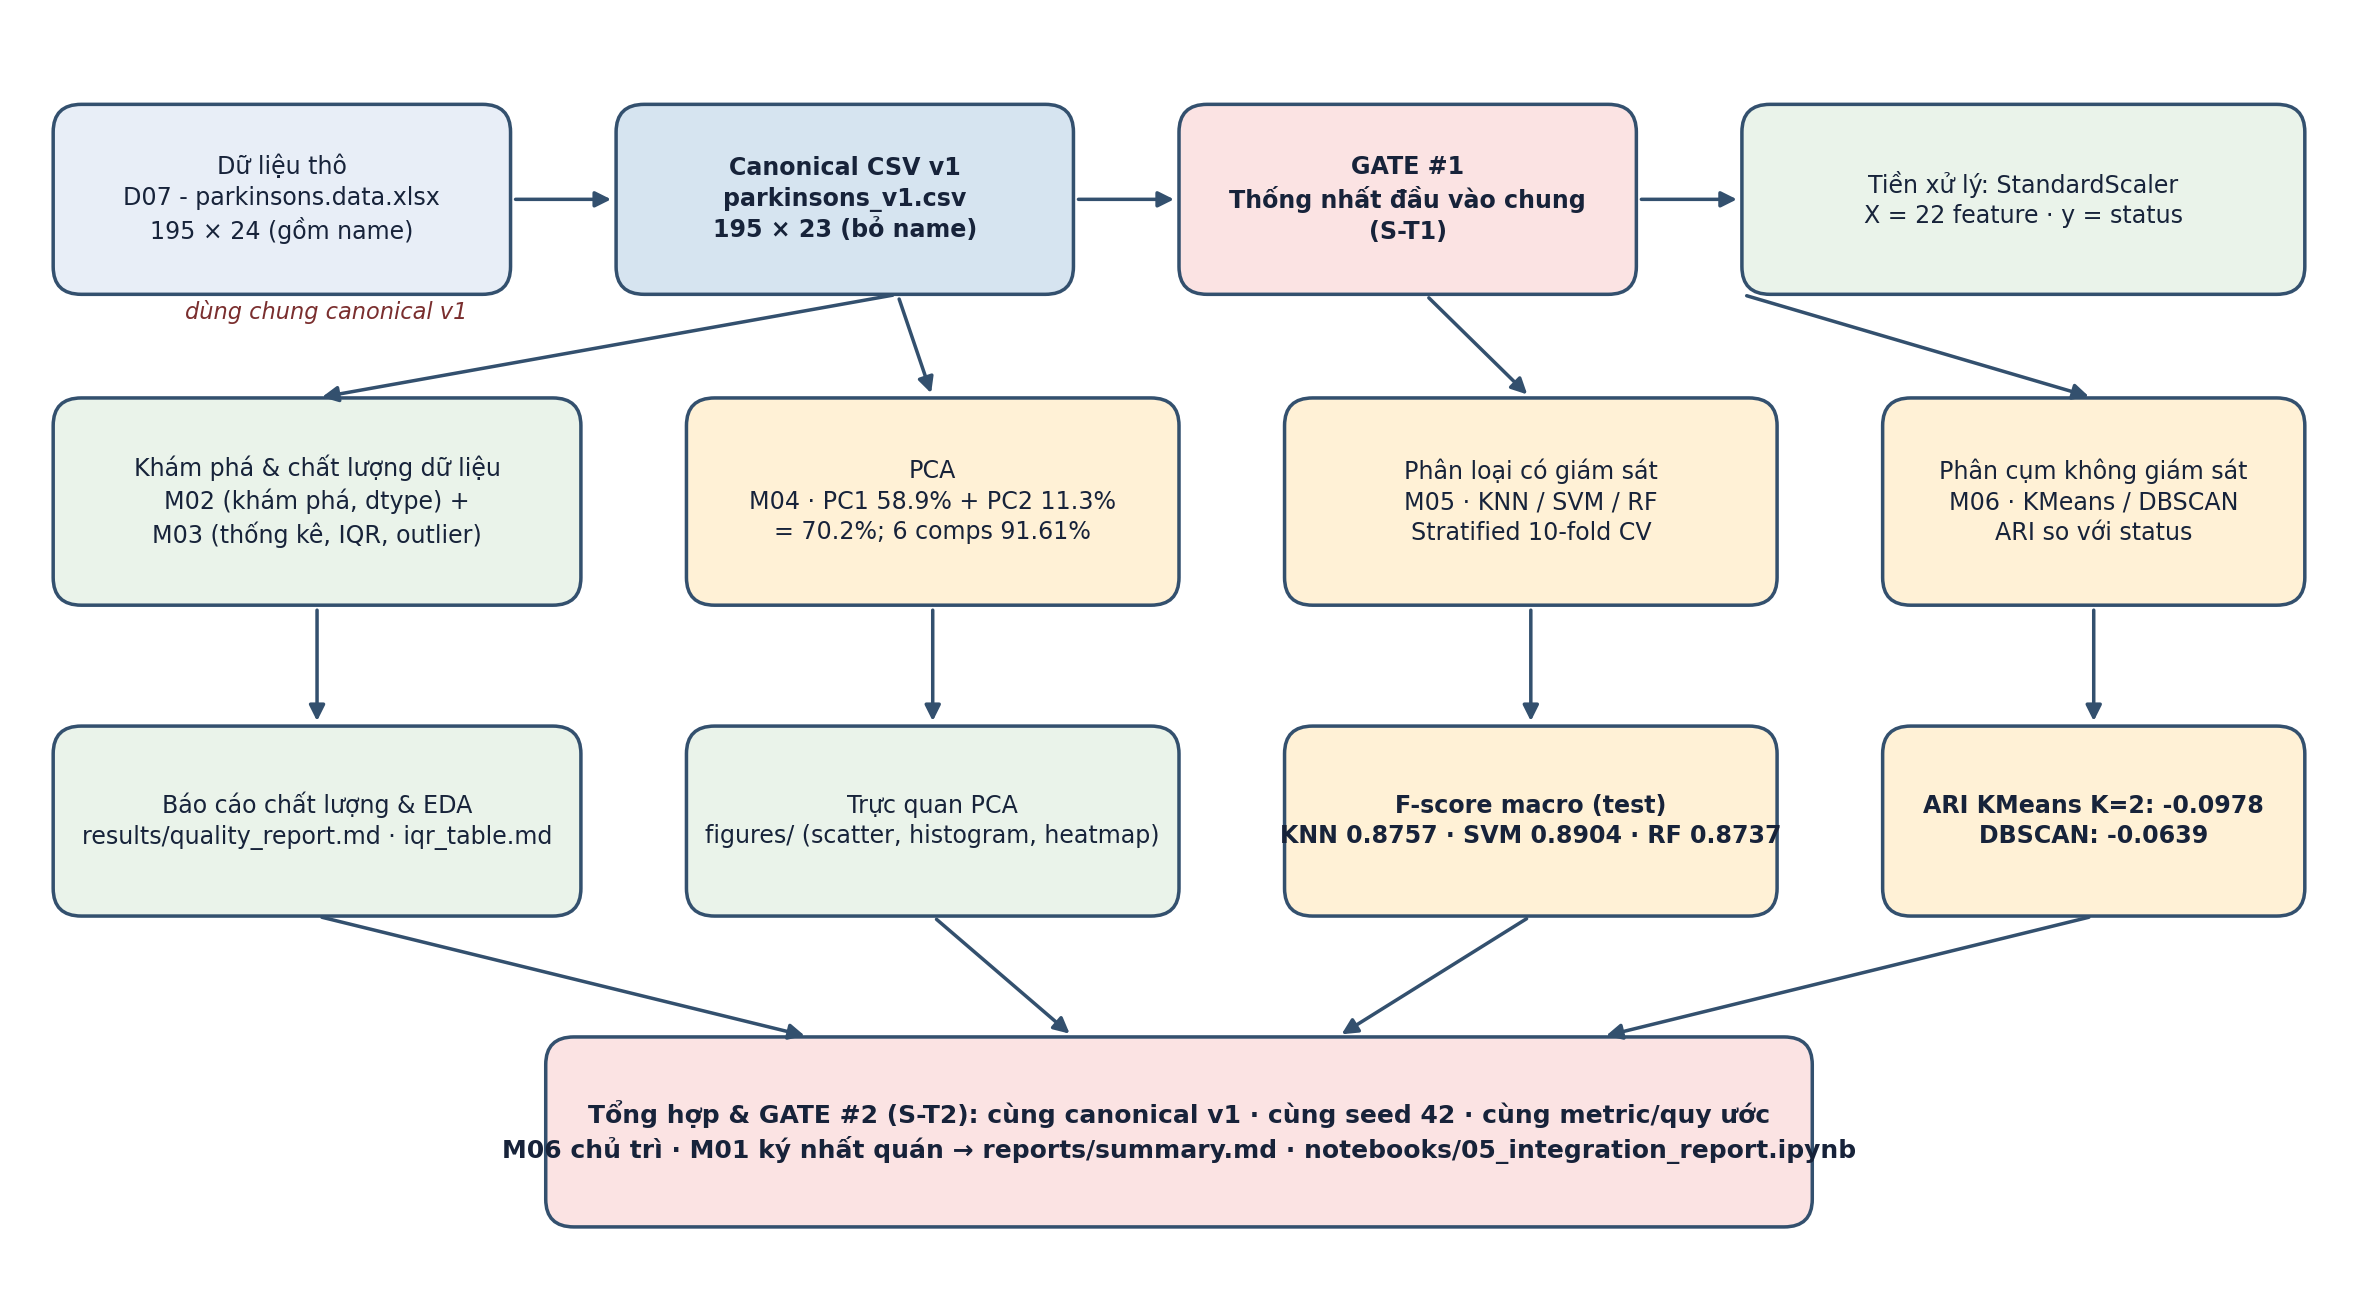
\includegraphics[width=\linewidth]{pipeline_diagram.png}
    \caption{Sơ đồ quy trình khai phá dữ liệu và các cổng kiểm soát}
    \label{fig:pipeline}
\end{figure}
\source{Tự biên soạn.}

Quy trình có hai cổng chất lượng bắt buộc:
\begin{itemize}
    \item \textbf{GATE \#1 (S-T1):} thống nhất đầu vào chuẩn \texttt{parkinsons\_v1.csv};
          các bước M02-M06 chỉ được chạy khi đầu ra của M01 đã sẵn sàng.
    \item \textbf{GATE \#2 (S-T2):} kiểm tra nhất quán toàn bộ số liệu trước khi tổng hợp,
          gồm cùng đầu vào, cùng seed, cùng độ đo và cùng quy ước.
\end{itemize}

\section{Dữ liệu và chuẩn hoá đầu vào}

\subsection{Nguồn dữ liệu}
Dữ liệu thô là tệp \texttt{D07 - parkinsons.data.xlsx} thu thập từ bộ dữ liệu Oxford
Parkinson's Disease Detection trên UCI \cite{uci_parkinsons}, gồm 195 bản ghi $\times$ 24 cột
(22 đặc trưng + nhãn \texttt{status} + cột định danh \texttt{name}). Nhóm loại bỏ cột
\texttt{name} (thông tin cá nhân) và giữ nguyên toàn bộ đặc trưng định lượng.

\subsection{Tạo bộ dữ liệu chuẩn (canonical CSV v1)}
Một tệp CSV duy nhất được sản xuất và đóng băng làm đầu vào cho mọi bước phân tích:

\begin{lstlisting}[language=Python, numbers=none]
data/processed/parkinsons_v1.csv
# 195 dong x 23 cot = 22 feature + status
# SHA-256: 55e2fed63eb74ad19a119b43ef33d92c
#          60d60f7d6751688f1cae45d38d358153
# SHA-256 tap tin tho (.xlsx):
# d5d96457a760cd06e93b1a1d1cd6380b
# 38909c2cc82121968bb51ef29f80029a
\end{lstlisting}

Việc này giúp tránh tình trạng các thành viên dùng lần lượt các phiên bản dữ liệu khác nhau
dẫn đến số liệu không thể đối chiếu. Cấu trúc đầu vào được mô tả đầy đủ trong
\texttt{data/processed/}\allowbreak\texttt{schema\_v1.md}.

\section{Kiến trúc thực hiện}

\subsection{Cấu trúc kho lưu trữ}

\begin{table}[H]
\centering
\caption{Cấu trúc chính của kho lưu trữ}
\begin{tabular}{|l|>{\raggedright\arraybackslash}p{8.6cm}|}
\hline
\textbf{Đường dẫn} & \textbf{Vai trò} \\
\hline
\texttt{data/raw/} & Dữ liệu thô và manifest nguồn \\
\hline
\texttt{data/processed/} & Canonical CSV v1 và schema \\
\hline
\texttt{notebooks/} & 5 notebook phân tích có lần lượt M01-M06 \\
\hline
\texttt{src/} & Hàm dùng chung và pipeline tổng hợp (\texttt{pipeline.py}) \\
\hline
\texttt{results/} & Báo cáo, bảng số liệu, hình ảnh, \texttt{pipeline\_summary.json} \\
\hline
\texttt{reports/} & Báo cáo tổng hợp cuối cùng \\
\hline
\texttt{workspaces/member-XX/} & Không gian làm việc của từng thành viên \\
\hline
\end{tabular}
\end{table}

\subsection{Pipeline tổng hợp}
Để kiểm chứng tính nhất quán, nhóm viết một lối chạy tổng hợp
(\texttt{python -m src.pipeline}) gọi lại các bước chuẩn bị dữ liệu, PCA và phân loại rồi
ghi kết quả vào \texttt{results/}\allowbreak\texttt{pipeline\_summary.json}. Lối chạy này không thay thế các
notebook chuyên sâu mà phục vụ đối chiếu chéo giữa các sản phẩm của nhóm.

\section{Quản lý công việc và đảm bảo chất lượng}

\subsection{Luồng Git và review}
Nhóm áp dụng luồng làm việc theo nhánh: mỗi nhiệm vụ tạo một nhánh riêng, mở pull request
(PR) về \texttt{main}, người phụ trách review bình luận và tag thành viên liên quan, chỉ
nhập nhánh sau khi có xác nhận đạt. Các PR đã merge bao gồm \#5 (khám phá), \#7 (tiền xử
lý-PCA), \#8 (phân loại), \#13 (thống kê/chất lượng), \#14 (phân cụm), \#16 (tổng hợp) và
\#17 (chốt gate). Đây là cách thức giúp mọi thay đổi đều được kiểm soát và truy vết.

\subsection{Bảng theo dõi nhiệm vụ}
Toàn bộ công việc được theo dõi trong \texttt{TASK\_BOARD.md} với 21 nhiệm vụ được mã hoá từ
M01-T1 tới S-T2. Mỗi nhiệm vụ chỉ được chuyển sang \texttt{Done} sau khi có bằng chứng đạt
review. Tại thời điểm tổng hợp, bảng ghi nhận \textbf{21/21 nhiệm vụ Done}; hai cổng GATE
\#1 và GATE \#2 đã được ký.

\subsection{Phân công và đóng góp}
Sáu thành viên phân công theo nhiệm vụ chính như Bảng \ref{tab:team_chap3}; nhóm điều phối
giữ vai trò cổng chất lượng, còn việc tổng hợp kết quả do hai thành viên M01 và M06 đồng sở
hữu để tránh phụ thuộc một người.

\begin{table}[H]
\centering
\caption{Phân công theo mô-đun và nghiệm thu}
\begin{tabular}{|c|l|l|}
\hline
\textbf{Mã} & \textbf{Họ và tên} & \textbf{Mô-đun / minh chứng nghiệm thu} \\
\hline
M01 & Đặng Hoàng Ân   & Dữ liệu, pipeline tổng hợp; ký GATE \#1, GATE \#2 \\
\hline
M02 & Lê Thiên Lộc    & M02-T1..T3; PR \#5 đạt review \\
\hline
M03 & Huỳnh Gia Hợp    & M03-T1..T3; PR \#13 đạt review \\
\hline
M04 & Trần Hoàng Thông & M04-T1..T3; PR \#7 đã merge \\
\hline
M05 & Ngô Thị Anh Thư   & M05-T1..T3; PR \#8 đạt review \\
\hline
M06 & Nguyễn Hoàng Bách & M06-T1..T3; PR \#14, PR \#16 đạt review \\
\hline
\end{tabular}
\label{tab:team_chap3}
\end{table}

\section{Môi trường thực nghiệm}

Thực nghiệm được thực hiện trên Python với các thư viện chuẩn của khoa học dữ liệu. Bảng
dưới ghi phiên bản được dùng ở lần chạy tổng hợp để cùng một cấu hình.

\begin{table}[H]
\centering
\caption{Môi trường thực nghiệm}
\begin{tabular}{|>{\raggedright\arraybackslash}p{5.2cm}|>{\raggedright\arraybackslash}p{10.2cm}|}
\hline
\textbf{Thành phần} & \textbf{Phiên bản / giá trị} \\
\hline
Python & 3.14.0 \\
\hline
numpy / pandas / scipy & 2.4.2 / 3.0.3 / 1.17.1 \\
\hline
scikit-learn & 1.9.0 \\
\hline
matplotlib / seaborn & 3.10.8 / 0.13.2 \\
\hline
Jupyter (nbformat, nbclient, nbconvert) & 5.11.1 / 0.11.0 / 7.17.2 \\
\hline
Hạt giống ngẫu nhiên & 42 \\
\hline
Kiểm định chéo & StratifiedKFold 10 (ngoài), GridSearchCV 5 (trong) \\
\hline
Độ đo chính & F-score macro (phân loại), ARI (phân cụm) \\
\hline
\end{tabular}
\end{table}

Các notebook M06 ban đầu chạy trên phiên bản thư viện khác (ví dụ scikit-learn 1.9.1);
kết quả vẫn khớp khi kiểm tra chéo, và nhóm đã ghi rõ phiên bản trong từng báo cáo để đảm
bảo minh bạch.

\section{Phương pháp đánh giá}

Với phân loại, hiệu năng được báo cáo dưới dạng trung bình $\pm$ độ lệch chuẩn của F-score
macro trên 10 fold kiểm tra, kèm F-score weighted và F-score trên tập huấn luyện để phát
hiện quá khớp. Với phân cụm, nhóm chọn số cụm K bằng silhouette, sau đó so sánh cụm với nhãn
bằng ARI; DBSCAN được chọn tham số bằng điểm uốn (knee) của khoảng cách láng giềng thứ
\texttt{min\_samples} và kiểm tra chéo trên lưới tham số. Mọi kết quả đều được ghi lại đầy
đủ trong thư mục \texttt{results/} kèm tham số, seed và phiên bản thư viện.

\chapter{KẾT QUẢ THỰC NGHIỆM}
\label{chap:results}

Chương này trình bày kết quả theo đúng trình tự nghiệm vụ: khám phá và chất lượng dữ
liệu (M02-M03), tiền xử lý với PCA (M04), phân loại có giám sát (M05) và phân cụm với
đánh giá ARI (M06). Mọi số liệu đều được tính trên \texttt{parkinsons\_v1.csv} và seed
\texttt{42}; minh chứng gốc nằm trong thư mục \texttt{results/}.

\section{Khám phá và chất lượng dữ liệu}

\subsection{Tổng quan dữ liệu}

\begin{table}[H]
\centering
\caption{Tổng quan dữ liệu canonical v1}
\begin{tabular}{|l|l|}
\hline
\textbf{Hạng mục} & \textbf{Giá trị} \\
\hline
Số mẫu $\times$ số cột & 195 $\times$ 23 (22 feature + \texttt{status}) \\
\hline
Giá trị thiếu / dòng trùng lặp & 0 / 0 \\
\hline
Nhãn \texttt{status=0} (khỏe) & 48 mẫu (24,62\%) \\
\hline
Nhãn \texttt{status=1} (Parkinson) & 147 mẫu (75,38\%) \\
\hline
Kiểu dữ liệu 22 feature & \texttt{float64}, phạm vi từ $7\times10^{-6}$ đến hàng trăm Hz \\
\hline
Feature có candidate outlier (IQR) & 19 / 22 \\
\hline
Mẫu có ít nhất một candidate outlier & 47 / 195 (24,10\%) \\
\hline
\end{tabular}
\end{table}

Dữ liệu sạch về thiếu và trùng lặp, nhưng mang hai đặc điểm cần xử lý: nhãn mất cân bằng
(theo chiều Parkinson) và thang đo các đặc trưng chênh lệch lớn. Các feature jitter có giá
trị rất nhỏ (ví dụ \texttt{MDVP:Jitter(\%)} dao động 0,0017-0,0332) trong khi
\texttt{MDVP:Fhi(Hz)} đạt 102-592, do đó việc chuẩn hoá là bắt buộc trước khi đưa vào mô
hình.

\begin{figure}[H]
    \centering
    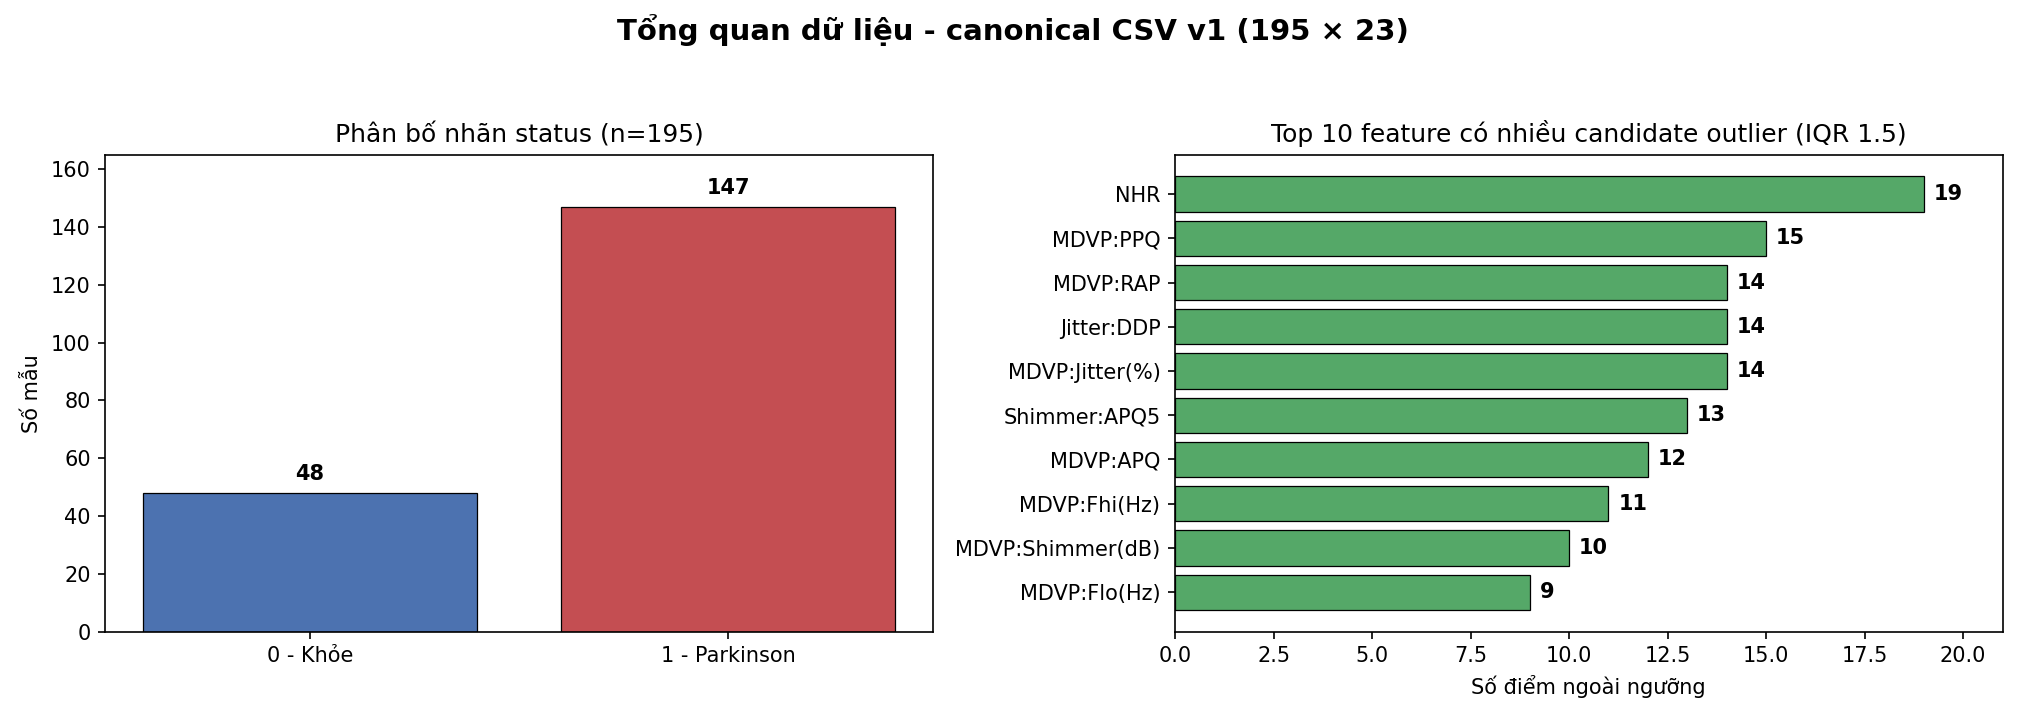
\includegraphics[width=\linewidth]{eda_summary.png}
    \caption{Phân bố nhãn \texttt{status} và các đặc trưng có nhiều candidate outlier theo IQR}
    \label{fig:eda}
\end{figure}
\source{Nhóm tổng hợp từ \texttt{results/quality\_report.md}.}

\subsection{Ngoại lai và độ lệch}

Theo quy tắc IQR hệ số 1,5, 19/22 feature xuất hiện giá trị ngoài ngưỡng; 47/195 mẫu
(24,10\%) chứa ít nhất một candidate outlier. Feature nổi bật là \texttt{NHR} (19 điểm,
9,74\%), \texttt{MDVP:PPQ} (15), các feature jitter \texttt{MDVP:RAP},
\texttt{Jitter:DDP}, \texttt{MDVP:Jitter(\%)} (14 mỗi cột) và \texttt{Shimmer:APQ5} (13).
Ba feature không có candidate outlier là \texttt{MDVP:Fo(Hz)}, \texttt{RPDE} và
\texttt{DFA}. Các điểm ngoại lai chủ yếu là biên độ cao thật của giọng bệnh, nhóm quyết
định giữ nguyên và kiểm soát rò rỉ thay vì loại bỏ mù quáng.

Độ lệch cho thấy 14/22 feature có $|\text{skew}| > 1$, riêng \texttt{NHR} có skew 4,2207
và kurtosis 21,9950, \texttt{MDVP:RAP}/\texttt{Jitter:DDP} skew khoảng 3,36. Đây là dấu
hiệu phân phối lệch mạnh ở nhóm nhiễu và jitter, phù hợp với bản chất của các đại lượng
âm học. Ngoài ra, 26/231 cặp feature có $|r| \ge 0{,}9$; hai cặp gần trùng thông tin là
\texttt{Jitter:DDP} $\approx 3\times$\texttt{MDVP:RAP} và
\texttt{Shimmer:DDA} $\approx 3\times$\texttt{Shimmer:APQ3} với $r = 1{,}0$. Canonical
CSV giữ nguyên các feature này để không thay đổi thông tin dữ liệu gốc.

\section{Tiền xử lý và phân tích thành phần chính}

\subsection{Chuẩn hoá và ma trận đặc trưng}
Nhóm tách $X$ (22 feature) và $y$ (\texttt{status}), sau đó chuẩn hoá z-score bằng
\texttt{StandardScaler}. Ma trận chuẩn hoá $X_s$ có kích thước $195\times22$, trung bình
gần 0 và độ lệch chuẩn gần 1, không có giá trị thiếu. Việc chuẩn hoá trên toàn bộ $X$ chỉ
dùng cho PCA và phân cụm; trong phân loại, bộ chuẩn hoá được đặt trong \texttt{Pipeline} để
fit riêng trên từng fold huấn luyện.

\subsection{Kết quả PCA}

\begin{table}[H]
\centering
\caption{Phương sai giải thích của PCA}
\begin{tabular}{|l|r|}
\hline
\textbf{Thành phần} & \textbf{Tỷ lệ phương sai giải thích} \\
\hline
PC1 & 58,9\% \\
\hline
PC2 & 11,3\% \\
\hline
PC1 + PC2 & 70,2\% \\
\hline
Thành phần đạt ngưỡng $\ge$ 90\% & 6 (tích luỹ 91,61\%) \\
\hline
\end{tabular}
\end{table}

Hai thành phần đầu giữ 70,2\% phương sai; để đạt ngưỡng 90\% phương sai cần 6 thành phần
(tích luỹ 91,61\%). Biểu đồ phân tán PC1-PC2 cho thấy hai nhóm tách một phần nhưng chồng
lấn đáng kể, tức ranh giới bệnh lý không nằm ngay trên hai trục chính.

\begin{figure}[H]
    \centering
    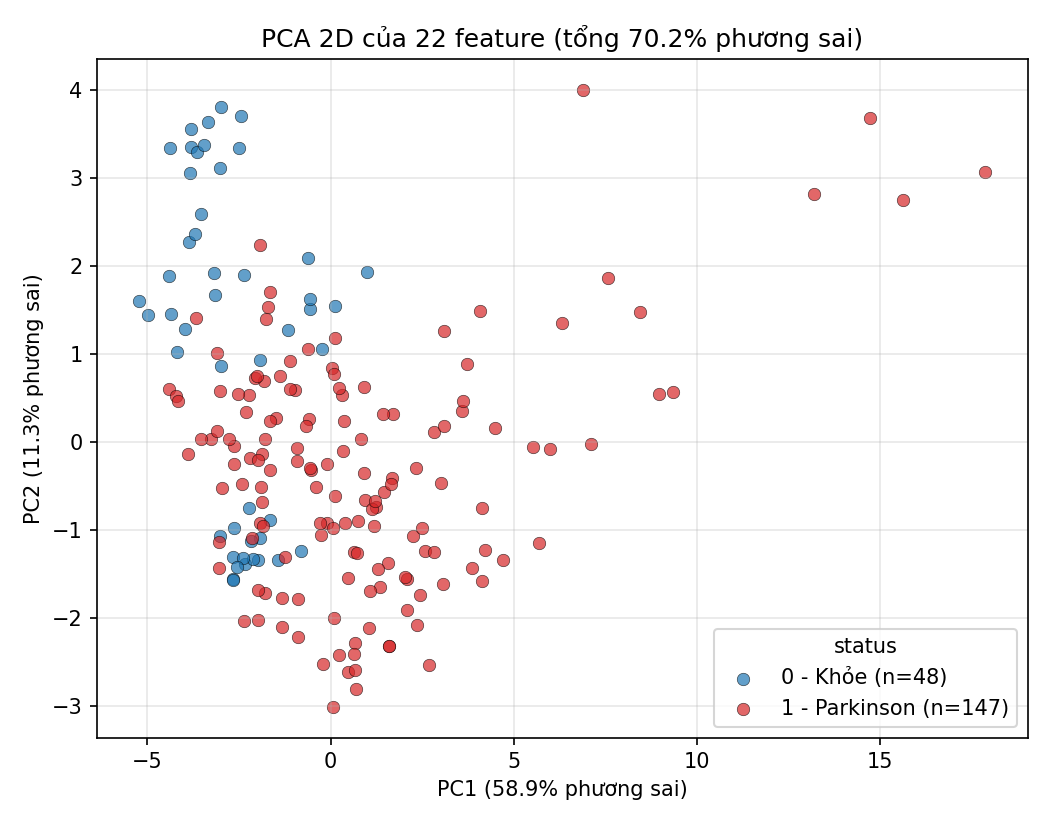
\includegraphics[width=0.78\linewidth]{pca_scatter.png}
    \caption{Scatter PC1-PC2 tô theo \texttt{status}}
    \label{fig:pca_scatter}
\end{figure}
\source{\texttt{results/figures/02\_pca\_scatter.png}.}

\begin{figure}[H]
    \centering
    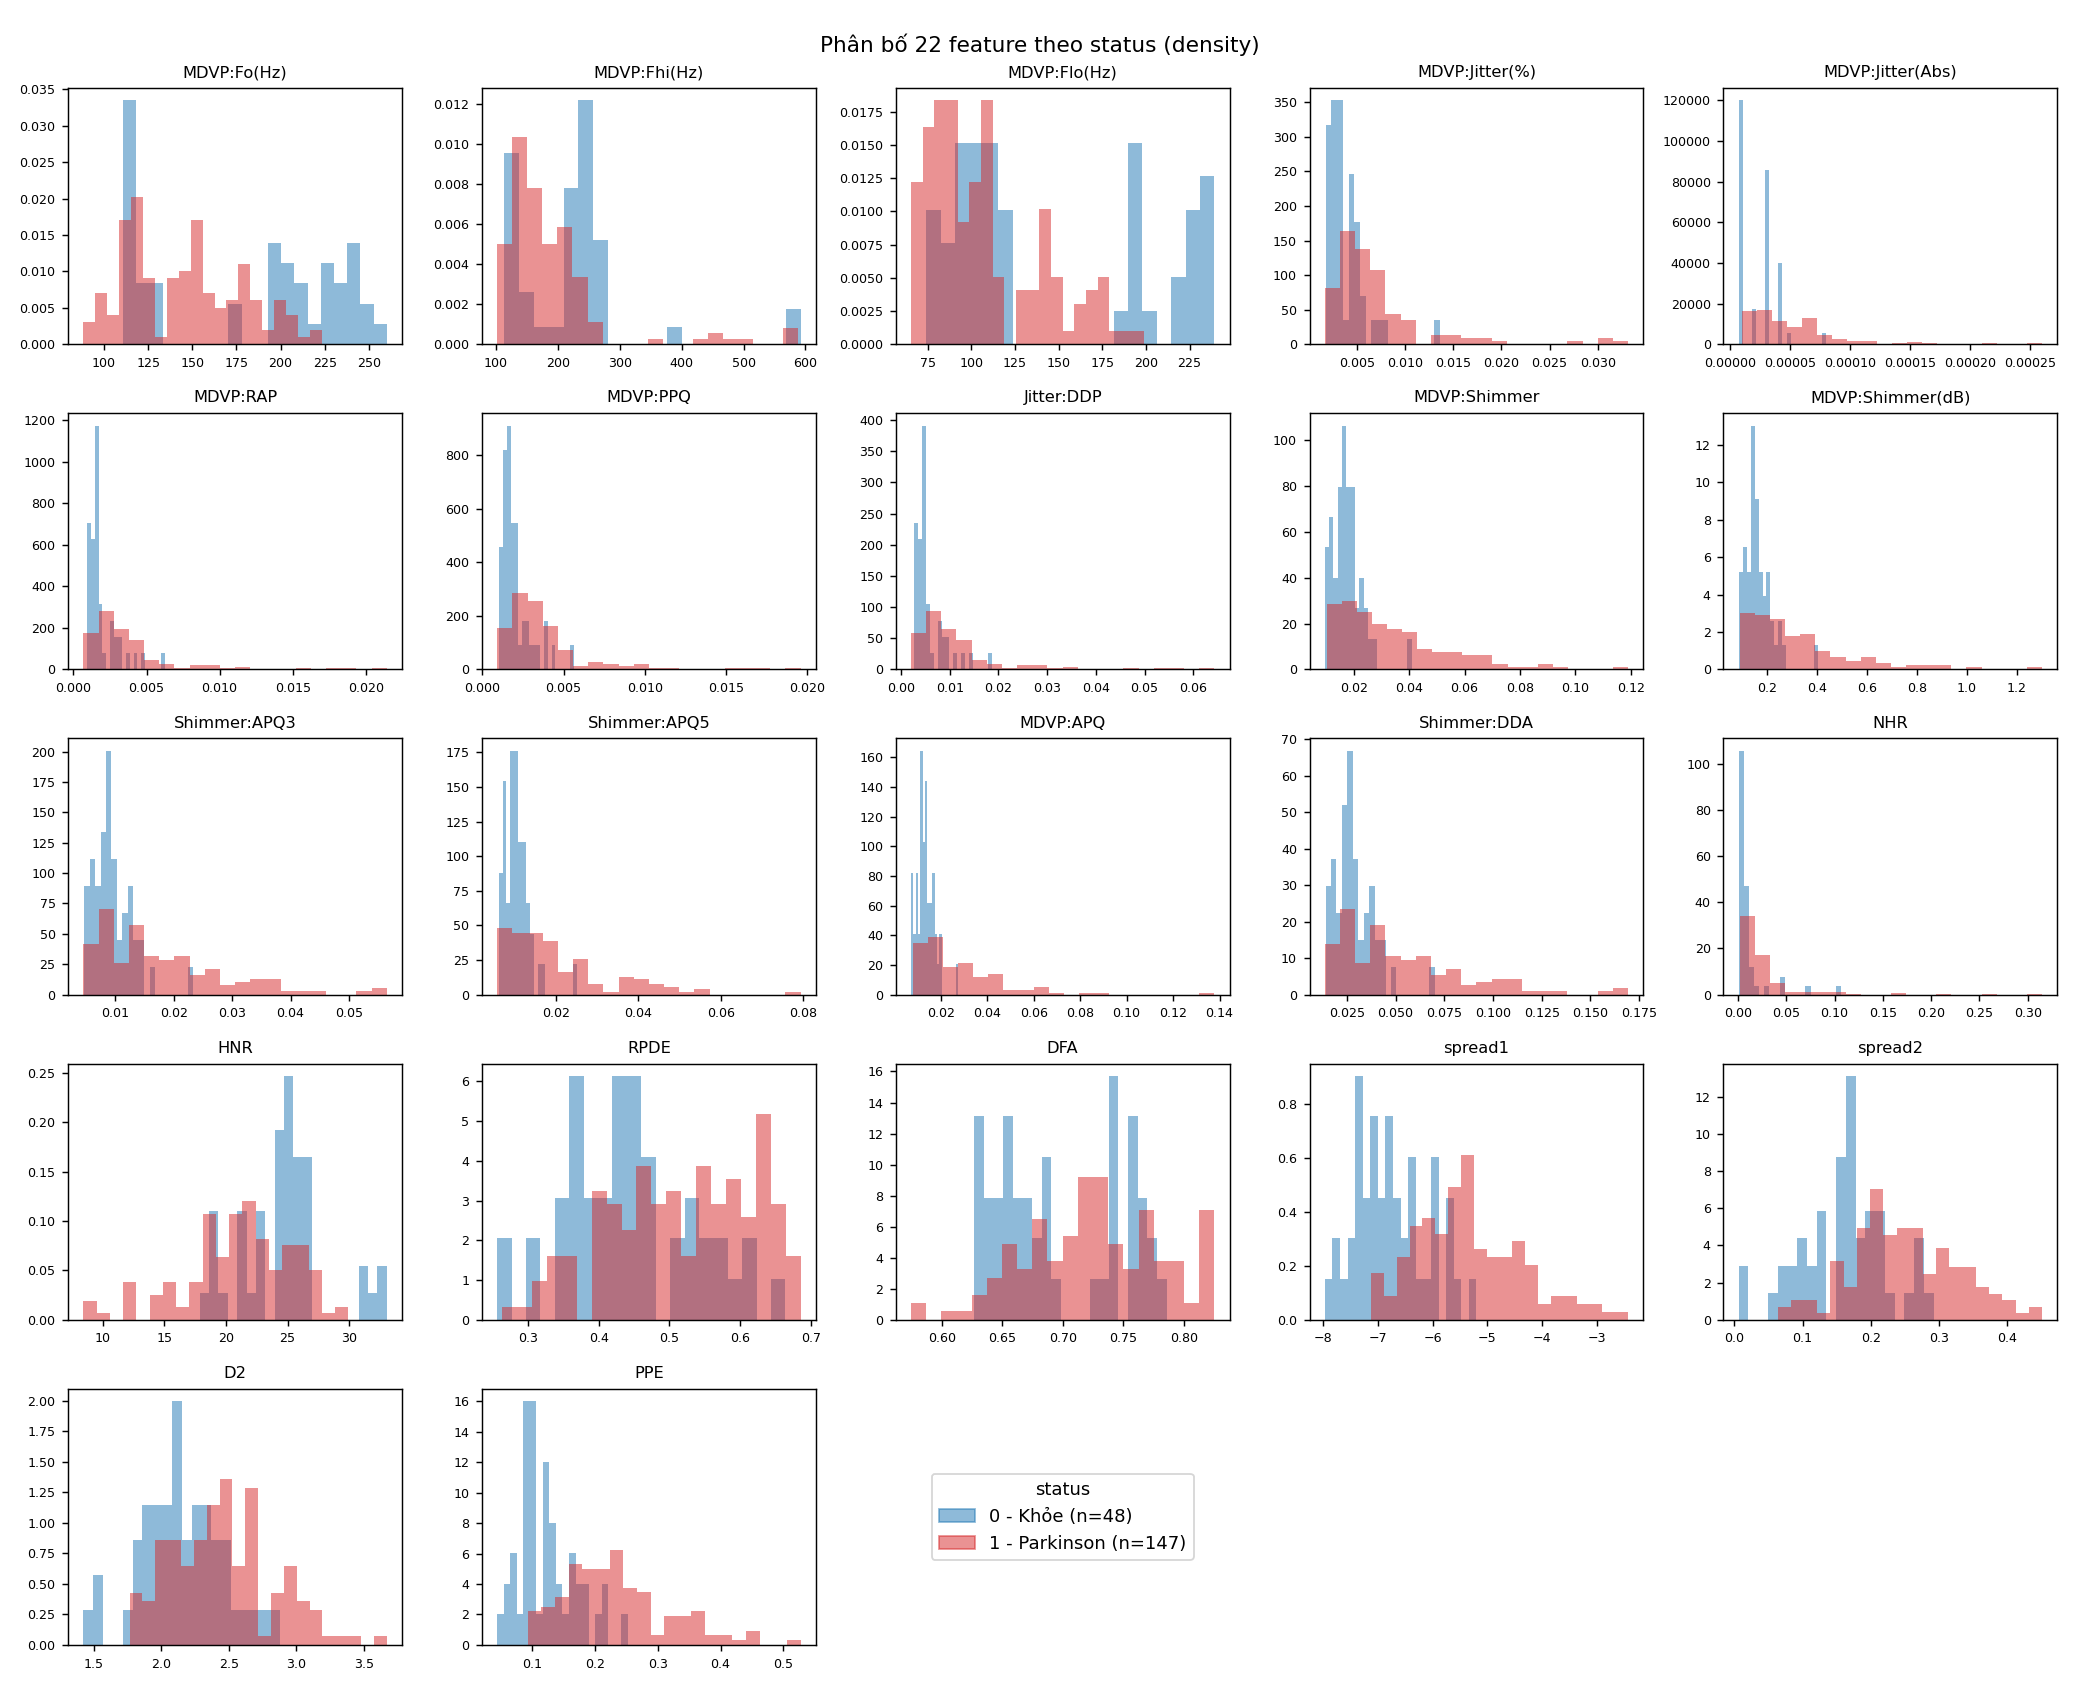
\includegraphics[width=0.84\linewidth]{histograms.png}
    \caption{Histogram 22 feature theo \texttt{status}}
    \label{fig:histograms}
\end{figure}
\source{\texttt{results/figures/m04-t3\_histograms.png}.}

\begin{figure}[H]
    \centering
    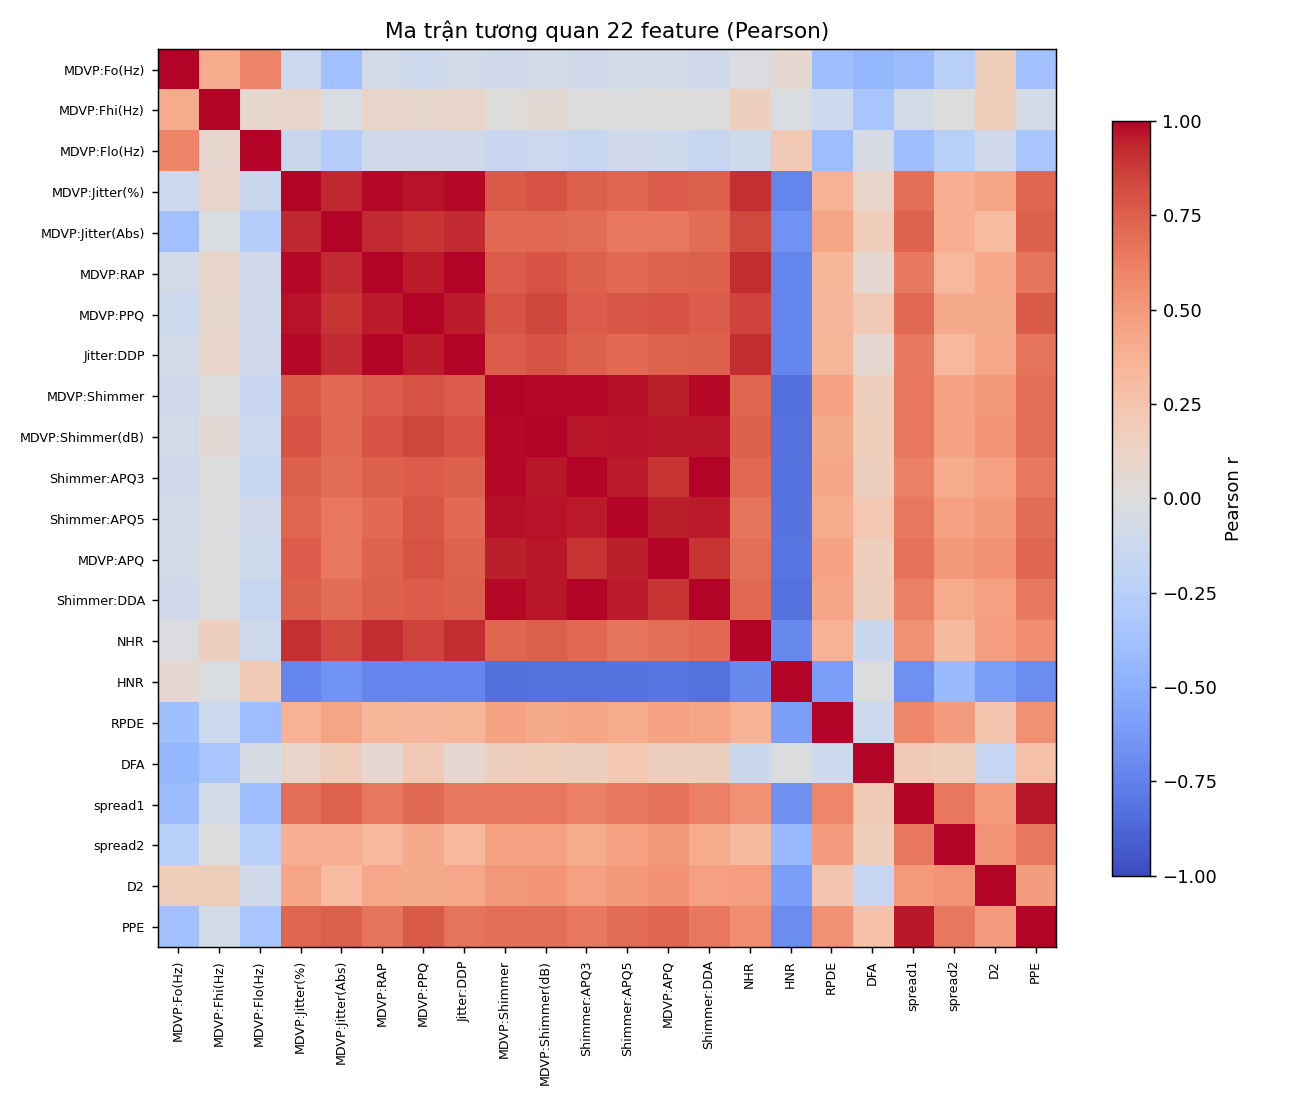
\includegraphics[width=0.84\linewidth]{corr_heatmap.png}
    \caption{Ma trận tương quan Pearson giữa các feature}
    \label{fig:heatmap}
\end{figure}
\source{\texttt{results/figures/m04-t3\_corr\_heatmap.png}.}

Histogram theo nhãn cho thấy nhiều feature có phân phối hai lớp chồng lấn, đặc biệt nhóm
jitter/shimmer; một số feature phi tuyến (RPDE, DFA, PPE) cho phân bố tách biệt hơn. Ma
trận tương quan xác nhận sự lặp thông tin trong nhóm jitter/shimmer như đã mô tả ở mục
trước.

\section{Phân loại có giám sát}

\subsection{Thiết lập thực nghiệm}
Nhóm dùng kiểm định chéo phân tầng 10-fold (seed 42), trong mỗi fold lại chạy tìm lưới 5-fold
trên tập huấn luyện; tiêu chí chọn tham số là F-score macro. Lưới tham số gồm KNN
$n\_neighbors \in \{3,5,7\}$, SVM $C \in \{0{,}1; 1; 10\}$ và Random Forest
$n\_estimators \in \{50; 100\}$. Bộ chuẩn hoá nằm trong \texttt{Pipeline}, fit trên phần
huấn luyện của từng fold.

\subsection{Kết quả}

\begin{table}[H]
\centering
\caption{F-score trên 10-fold CV (mean $\pm$ std)}
\begin{tabular}{|l|c|c|c|}
\hline
\textbf{Mô hình} & \textbf{F-score macro (test)} & \textbf{F-score weighted (test)} & \textbf{F-score macro (train)} \\
\hline
KNN & 0,8757 $\pm$ 0,0742 & 0,9073 $\pm$ 0,0578 & 0,9647 \\
\hline
SVM & \textbf{0,8904 $\pm$ 0,0804} & \textbf{0,9199 $\pm$ 0,0603} & 0,9787 \\
\hline
Random Forest & 0,8737 $\pm$ 0,1171 & 0,9103 $\pm$ 0,0824 & 1,0000 \\
\hline
\end{tabular}
\end{table}

\begin{figure}[H]
    \centering
    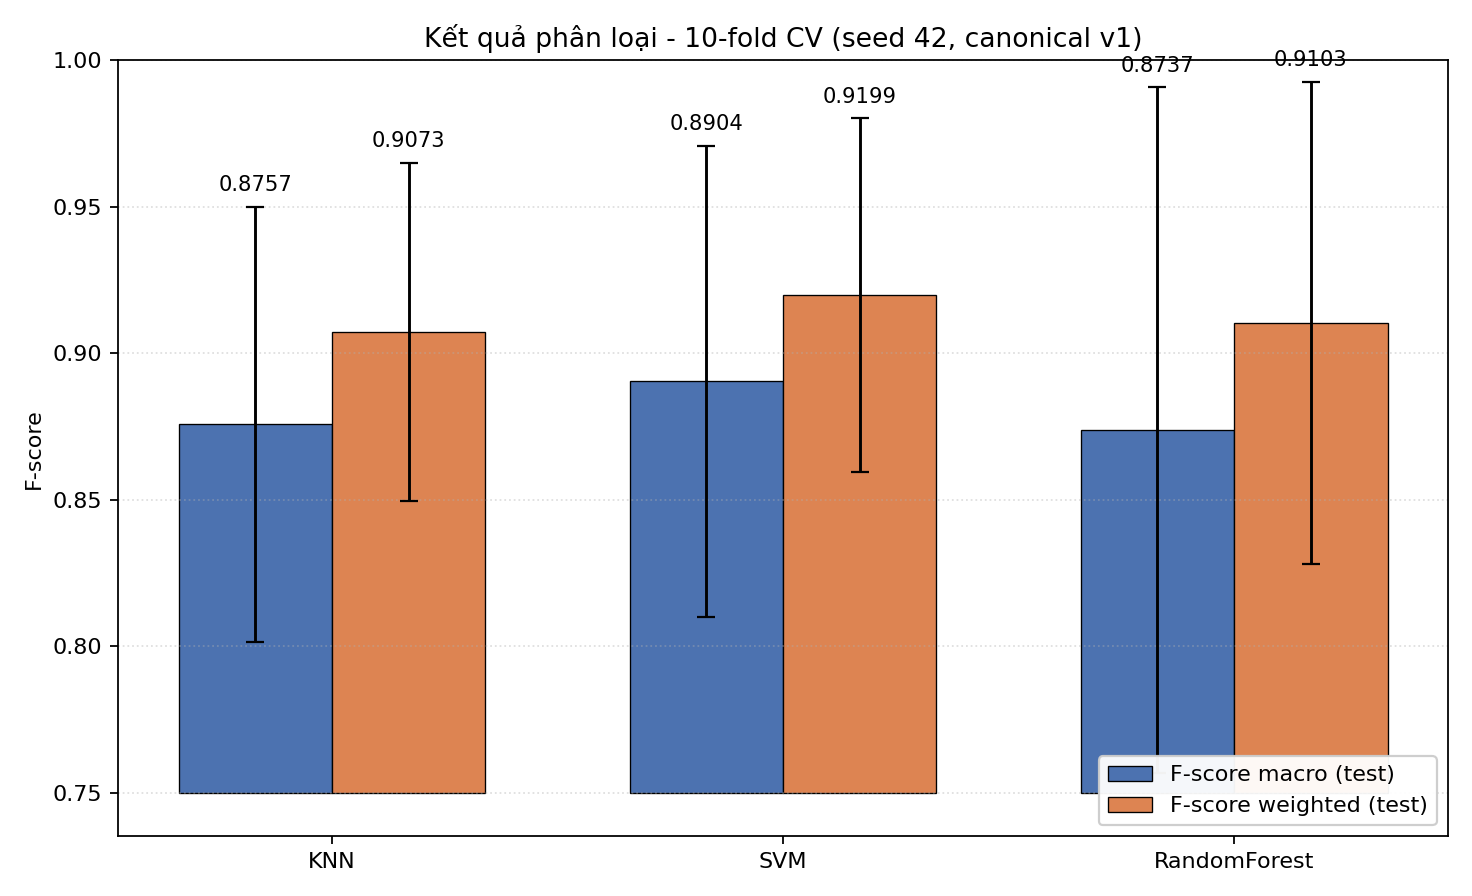
\includegraphics[width=0.86\linewidth]{f1_scores.png}
    \caption{F-score macro và weighted trên 10-fold CV cho ba mô hình}
    \label{fig:f1}
\end{figure}
\source{\texttt{docs/images/f1\_scores.png}.}

Ba mô hình đều đạt F-score macro trên 0,87 trên tập kiểm tra. SVM đạt cao nhất (0,8904),
nhưng chênh lệch giữa các mô hình chỉ khoảng 0,016 - nhỏ hơn độ lệch chuẩn giữa các fold
(0,07-0,12) - do đó báo cáo không kết luận một mô hình tốt nhất một cách chắc chắn.
F-score weighted cao hơn macro ở cả ba mô hình do lớp khỏe (48 mẫu) có tỷ trọng nhỏ.
Random Forest có điểm huấn luyện 1,0000 và độ lệch chuẩn lớn nhất, cho thấy dấu hiệu quá
khớp; KNN và SVM ổn định hơn.

\section{Phân cụm không giám sát và đánh giá ARI}

\subsection{K-Means}
Các mô hình K-Means ($K = 2\dots10$, $n\_init=10$, seed 42) được chạy trên $X_s$; số cụm
được chọn theo silhouette trung bình. Kết quả đầy đủ ở Bảng \ref{tab:kmeans}.

\begin{table}[H]
\centering
\caption{Kết quả K-Means và ARI so với \texttt{status}}
\begin{tabular}{|c|r|r|l|r|}
\hline
\textbf{K} & \textbf{Inertia} & \textbf{Silhouette} & \textbf{Kích thước cụm} & \textbf{ARI} \\
\hline
\textbf{2} & 2817,2 & \textbf{0,4373} & [165, 30] & \textbf{$-$0,0978} \\
\hline
3 & 2076,2 & 0,2763 & [106, 77, 12] & 0,0582 \\
\hline
4 & 1822,4 & 0,2358 & [91, 77, 23, 4] & 0,0583 \\
\hline
5 & 1595,5 & 0,2048 & [73, 64, 32, 22, 4] & 0,1000 \\
\hline
6 & 1442,0 & 0,2138 & [60, 51, 30, 28, 22, 4] & 0,1058 \\
\hline
7 & 1319,8 & 0,2094 & [54, 51, 31, 24, 23, 8, 4] & 0,0882 \\
\hline
8 & 1230,5 & 0,2201 & [53, 35, 32, 23, 23, 15, 10, 4] & 0,0313 \\
\hline
9 & 1157,0 & 0,2265 & [52, 39, 25, 24, 21, 13, 9, 8, 4] & 0,0574 \\
\hline
10 & 1110,7 & 0,1896 & [38, 35, 26, 23, 22, 18, 12, 9, 8, 4] & 0,0481 \\
\hline
\end{tabular}
\label{tab:kmeans}
\end{table}

Silhouette đạt cực đại tại $K = 2$ (0,4373), giảm mạnh ở $K = 3$ (0,2763) và dao động quanh
0,19-0,24 ở các giá trị lớn hơn; đường cong inertia giảm đều, không có điểm gập rõ ràng nên
Elbow chỉ dùng để đối chiếu. Tuy nhiên, ARI tại $K = 2$ là $-0{,}0978$ và trên toàn dải
$K$ chỉ nằm trong $[-0{,}0978; 0{,}1058]$, cho thấy cụm K-Means không khớp ranh giới bệnh
lý. Cụm nhỏ 30 mẫu nằm lệch về phía PC1 dương, nhiều khả năng là nhóm có biên độ cao
thay vì nhóm khỏe mạnh.

\begin{figure}[H]
    \centering
    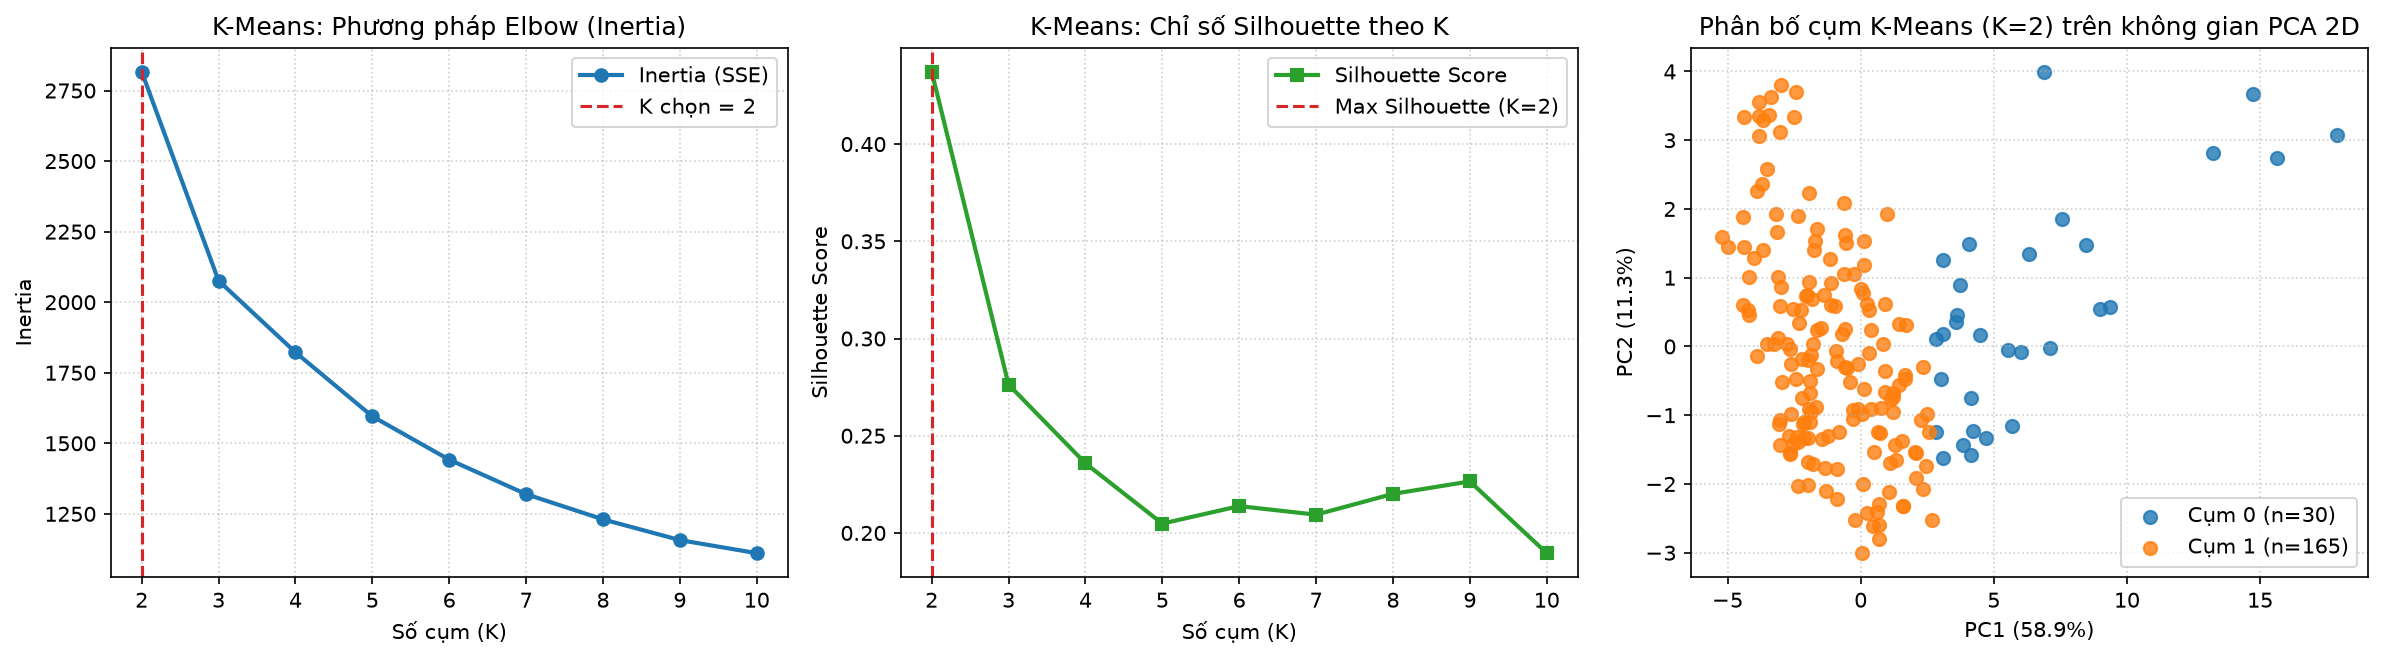
\includegraphics[width=0.92\linewidth]{kmeans_selection.png}
    \caption{Đánh giá K-Means: inertia, silhouette và kích thước cụm theo K}
    \label{fig:kmeans}
\end{figure}
\source{\texttt{results/figures/m06\_kmeans\_selection.png}.}

\subsection{DBSCAN}
Với \texttt{min\_samples = 5}, đường cong k-distance cho điểm uốn tại $\varepsilon = 3{,}37$.
DBSCAN tại cấu hình này tạo \textbf{một} cụm gồm 183 điểm và 12 điểm nhiễu, với ARI
$-0{,}0639$. Khảo sát lưới tham số
($\varepsilon \in \{1{,}5; 2{,}0; 2{,}5; 3{,}0; 3{,}5; 4{,}0; 5{,}0\}$,
\texttt{min\_samples} $\in \{3; 5; 10\}$) cho thấy ARI chỉ nằm trong
$[-0{,}0744; 0{,}1625]$; giá trị cao nhất 0,1625 đạt khi $\varepsilon = 1{,}5$,
\texttt{min\_samples} = 5 nhưng khi đó 149/195 điểm là nhiễu, không có ý nghĩa phân cụm.
Kết quả cho thấy trong không gian 22 chiều chuẩn hoá, mật độ điểm phân bố liên tục và
không hình thành các vùng mật độ tách biệt ứng với hai lớp bệnh/khỏe.

\begin{figure}[H]
    \centering
    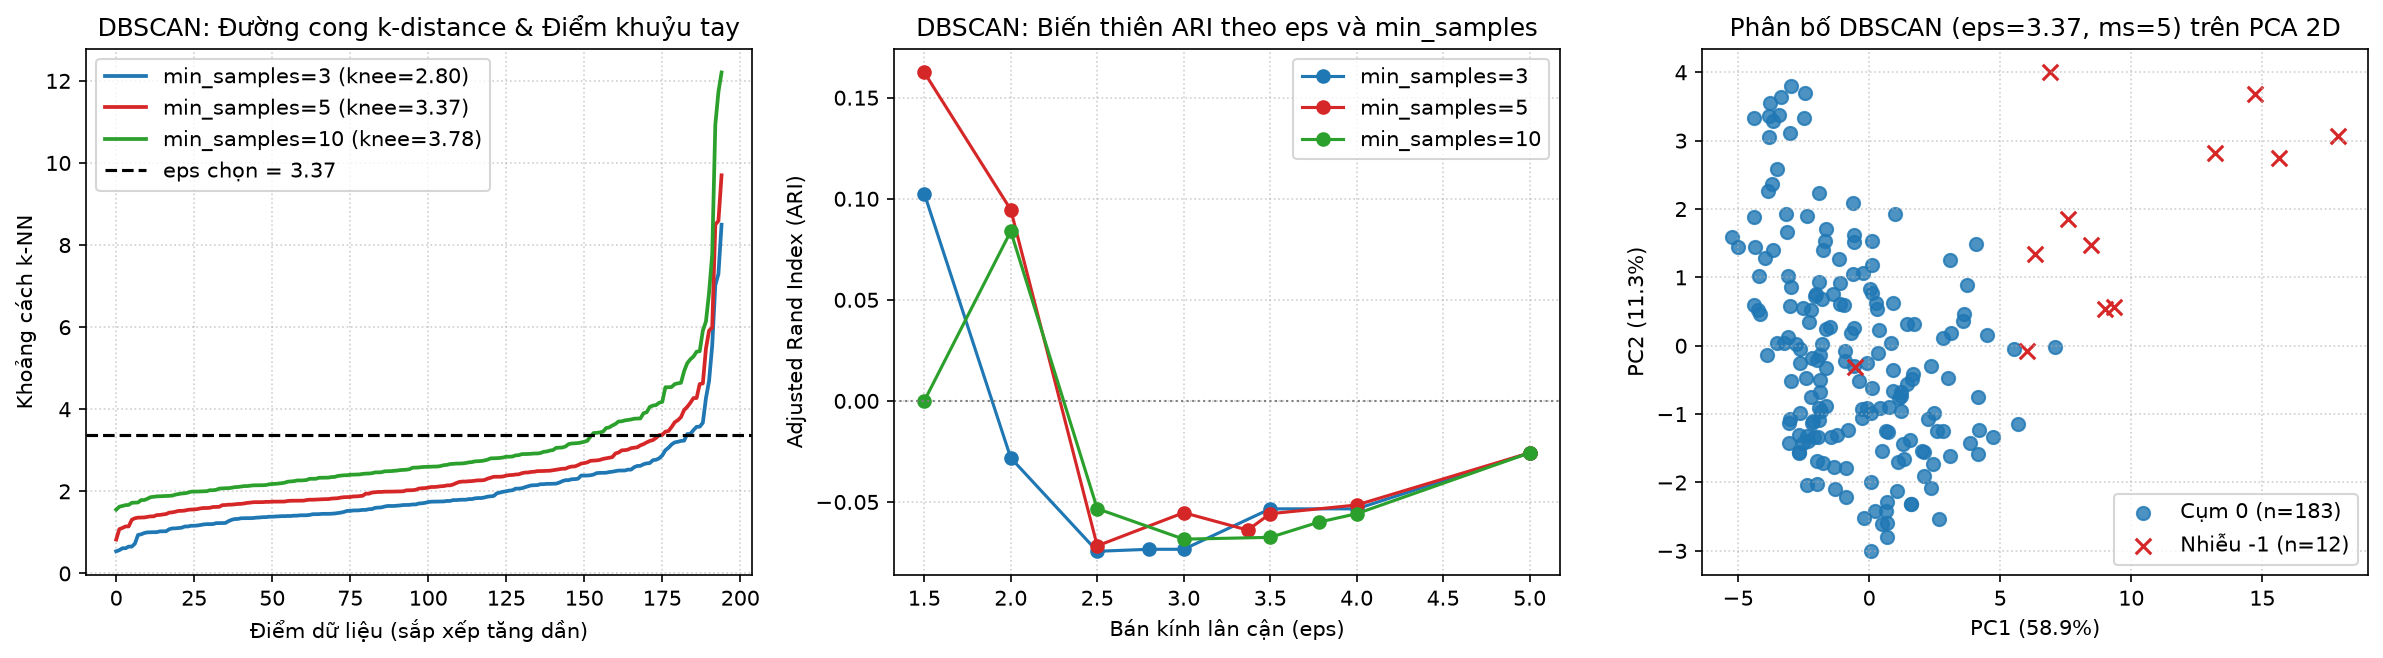
\includegraphics[width=0.92\linewidth]{dbscan_analysis.png}
    \caption{Phân tích DBSCAN: k-distance, cụm/nhiễu và ARI theo tham số}
    \label{fig:dbscan}
\end{figure}
\source{\texttt{results/figures/m06\_dbscan\_analysis.png}.}

\section{Đối chiếu tổng hợp}

\begin{table}[H]
\centering
\caption{Đối chiếu câu hỏi nghiên cứu với kết quả}
\begin{tabular}{|p{1.6cm}|p{6.2cm}|p{6.4cm}|}
\hline
\textbf{Câu hỏi} & \textbf{Kết quả chính} & \textbf{Nhận xét} \\
\hline
RQ1 & 0 NaN/trùng; 19/22 feature có outlier IQR; 47/195 mẫu; nhãn 147/48; 14/22 feature lệch mạnh & Dữ liệu sạch nhưng lệch nhãn/thang đo; cần chuẩn hoá và CV phân tầng \\
\hline
RQ2 & F-score macro 0,8757 (KNN), 0,8904 (SVM), 0,8737 (RF); RF có dấu hiệu quá khớp & Phân loại đạt tốt; chênh lệch giữa mô hình nhỏ so với biến động giữa fold \\
\hline
RQ3 & K-Means K=2 silhouette 0,4373 nhưng ARI $-$0,0978; DBSCAN 1 cụm, 12 nhiễu, ARI $-$0,0639 & Cấu trúc cụm không khớp \texttt{status}; bệnh lý cần mô hình có giám sát \\
\hline
\end{tabular}
\end{table}

Kết quả cho thấy quy trình khai phá dữ liệu vận hành nhất quán: dữ liệu đầu vào duy nhất,
mọi bước tái lập với seed 42, và các kết luận được giới hạn đúng theo độ biến động của số
liệu. Phân loại có giám sát giữ vai trò chính trong bài toán, trong khi phân cụm phục vụ
đối chiếu và nhận định giới hạn của tín hiệu không gian đặc trưng.

\chapter{KẾT LUẬN VÀ HƯỚNG PHÁT TRIỂN}
\label{chap:conclusion}

\section{Kết luận}

Nhóm đã hoàn thành quy trình khai phá dữ liệu hoàn chỉnh trên bộ dữ liệu giọng nói
Parkinson của UCI, với ba câu hỏi nghiên cứu được trả lời như sau.

\textbf{RQ1 -- Chất lượng dữ liệu.} Bộ dữ liệu canonical gồm 195 bản ghi $\times$ 23 cột,
không có giá trị thiếu hay dòng trùng lặp. Nhãn mất cân bằng (147 Parkinson / 48 khỏe),
thang đo đặc trưng chênh lệch lớn, 19/22 feature có candidate outlier theo IQR và 47/195
mẫu chứa ít nhất một candidate outlier; 14/22 feature có độ lệch $|\text{skew}| > 1$. Từ
đó nhóm áp dụng chuẩn hoá z-score và kiểm định chéo phân tầng để giảm ảnh hưởng của hai
đặc điểm này.

\textbf{RQ2 -- Phân loại có giám sát.} Trên 10-fold CV, ba mô hình đạt F-score macro 0,8757
(KNN), 0,8904 (SVM) và 0,8737 (Random Forest). SVM có kết quả cao nhất nhưng chênh lệch
giữa các mô hình nhỏ so với độ biến động giữa các fold; Random Forest cho thấy dấu hiệu
quá khớp (F-score huấn luyện 1,0000). Kết quả cho thấy tín hiệu giọng nói mang thông tin
phân biệt bệnh lý ở mức tốt.

\textbf{RQ3 -- Phân cụm không giám sát.} K-Means chọn $K=2$ theo silhouette (0,4373) nhưng
ARI chỉ $-0{,}0978$; DBSCAN đạt $\varepsilon = 3{,}37$, \texttt{min\_samples} = 5 cho một
cụm lớn, 12 điểm nhiễu và ARI $-0{,}0639$. Cấu trúc cụm trong không gian 22 đặc trưng do
đó không khớp ranh giới bệnh lý \texttt{status}; phân cụm đóng vai trò đối chiếu, không thay
thế mô hình có giám sát.

Ngoài kết quả kỹ thuật, đề tài còn rèn được quy trình làm việc nhóm: quản lý mã nguồn theo
nhánh, review từng pull request, đóng băng đầu vào chuẩn và chốt hai cổng GATE để đảm bảo
mọi kết quả nhất quán, tái lập được.

\section{Hạn chế}

\begin{itemize}
    \item Mẫu nhỏ (195 bản ghi, khoảng 32 chủ thể theo mô tả UCI) và mất cân bằng nhãn; mỗi
          fold kiểm tra chỉ khoảng 20 mẫu, trong đó khoảng 5 mẫu lớp khỏe nên điểm số giữa
          các fold dao động lớn.
    \item Cột \texttt{name} đã được loại khỏi canonical CSV nên không thực hiện kiểm định
          chéo theo nhóm chủ thể; bản ghi của cùng một người có thể rơi vào cả huấn luyện và
          kiểm tra, khiến điểm test có thể cao hơn thực tế.
    \item PCA hai chiều chỉ giữ 70,2\% phương sai; phân cụm không tách được cấu trúc khớp
          nhãn, DBSCAN chỉ tạo một cụm lớn với 12 điểm nhiễu.
    \item Mới so sánh ba mô hình với lưới tham số nhỏ; chưa tinh chỉnh ngưỡng quyết định,
          chưa huấn luyện trên tập dữ liệu độc lập.
    \item Một số thành viên chạy trên phiên bản thư viện khác nhau (ví dụ scikit-learn
          1.9.1); số liệu vẫn khớp khi kiểm tra chéo nhưng lần chạy cần ghi rõ môi trường.
\end{itemize}

\section{Hướng phát triển}

\begin{itemize}
    \item Bổ sung đặc trưng, lựa chọn đặc trưng (feature selection) và thử nghiệm thêm các
          mô hình hiện đại hơn; nghiên cứu kiểm định chéo theo nhóm chủ thể
          (\texttt{GroupKFold}) để khắc phục rò rỉ theo người.
    \item Điều chỉnh đơn vị/nhãn lưỡng phân hóa (threshold, class-weight) phù hợp với mục
          tiêu sàng lọc; đánh giá thêm độ tin cậy (calibration) và toàn diện (độ nhạy, độ
          đặc hiệu).
    \item Kết hợp nhãn với phân cụm (semi-supervised) hoặc học sâu trên tín hiệu âm thanh
          thô, và xây dựng giao diện nhỏ minh hoạ pipeline cho người dùng.
    \item Hoàn thiện hạ tầng tái lập: khóa phiên bản thư viện, thêm kiểm tra tự động cho
          dữ liệu đầu vào và đầu ra, chạy pipeline bằng một lệnh duy nhất.
\end{itemize}

\section{Đóng góp của nhóm và nghiệm thu}

Toàn bộ 21 nhiệm vụ trong bảng theo dõi đã được thực hiện và nghiệm thu \textbf{Done};
hai cổng GATE \#1 và GATE \#2 đã ký. Các pull request đã merge gồm \#5, \#7, \#8, \#13,
\#14, \#16 và \#17; mỗi nhiệm vụ chỉ được đóng sau khi có review độc lập.

\begin{table}[H]
\centering
\caption{Trạng thái nghiệm thu của từng thành viên}
\begin{tabular}{|c|l|l|}
\hline
\textbf{Mã} & \textbf{Thành viên} & \textbf{Trạng thái / bằng chứng} \\
\hline
M01 & Đặng Hoàng Ân   & Hoàn thành; ký GATE \#1, GATE \#2 \\
\hline
M02 & Lê Thiên Lộc    & Hoàn thành; PR \#5 đạt review \\
\hline
M03 & Huỳnh Gia Hợp    & Hoàn thành; PR \#13 đạt review \\
\hline
M04 & Trần Hoàng Thông & Hoàn thành; PR \#7 đã merge \\
\hline
M05 & Ngô Thị Anh Thư   & Hoàn thành; PR \#8 đạt review \\
\hline
M06 & Nguyễn Hoàng Bách & Hoàn thành; PR \#14, \#16 đạt review \\
\hline
\end{tabular}
\end{table}

Nhóm hy vọng báo cáo đáp ứng yêu cầu môn Khai phá dữ liệu; mọi thiếu sót còn lại nhóm sẽ
bổ sung theo hướng dẫn của giảng viên.


% ---------- 5. TÀI LIỆU THAM KHẢO ----------
\cleardoublepage
\addcontentsline{toc}{chapter}{\bibname}
\bibliographystyle{ieeetr-hyphen}
\bibliography{refs}

% ---------- 6. PHỤ LỤC ----------
\cleardoublepage
\appendix
\chapter{KHO LƯU TRỮ, CẤU TRÚC VÀ CÁCH TÁI LẬP}
\label{app:a}

\section{Kho lưu trữ mã nguồn}

Toàn bộ mã nguồn, dữ liệu đã xử lý, notebook và kết quả được lưu trữ tại:
\begin{center}
    \url{https://github.com/KaiyoDev/Nhom_3_KhaiThacDuLieu_Parkinsons}
\end{center}

Nhánh \texttt{main} chứa các sản phẩm đã nghiệm thu; lịch sử thay đổi và review được theo
dõi trong các pull request \#5, \#7, \#8, \#13, \#14, \#16 và \#17.

\section{Cấu trúc thư mục chính}

\begin{table}[H]
\centering
\begin{tabular}{|l|p{8.4cm}|}
\hline
\textbf{Đường dẫn} & \textbf{Nội dung} \\
\hline
\texttt{data/raw/} & Tệp thô \texttt{D07 - parkinsons.data.xlsx}, manifest \\
\hline
\texttt{data/processed/} & \texttt{parkinsons\_v1.csv} (canonical), \texttt{schema\_v1.md} \\
\hline
\texttt{notebooks/} & 01 exploration, 02 preprocessing+PCA, 03 classification, 04 clustering, 05 integration report \\
\hline
\texttt{src/} & \texttt{preprocessing.py}, \texttt{pipeline.py} \\
\hline
\texttt{results/} & Báo cáo, bảng số liệu CSV, hình ảnh, \texttt{pipeline\_summary.json} \\
\hline
\texttt{reports/summary.md} & Báo cáo tổng hợp đa nhiệm vụ \\
\hline
\end{tabular}
\end{table}

\section{Cách tái lập}

Yêu cầu: Python 3.10+, cài các gói trong \texttt{requirements.txt}. Trong thư mục gốc:

\begin{lstlisting}[language=bash, numbers=none]
pip install -r requirements.txt
python -m src.pipeline          # ghi results/pipeline_summary.json
jupyter nbconvert -to notebook -execute notebooks/05_integration_report.ipynb
\end{lstlisting}

Quy ước cố định: seed \texttt{42}; kiểm định chéo ngoài 10 fold, trong 5 fold;
\texttt{StandardScaler}; độ đo chính là F-score macro (phân loại) và ARI (phân cụm);
PCA 2 thành phần để trực quan hoá, 6 thành phần để đạt $\ge$ 90\% phương sai.

\section{Thông tin nhóm}

\begin{table}[H]
\centering
\begin{tabular}{|c|l|l|l|}
\hline
\textbf{Mã} & \textbf{Họ và tên} & \textbf{MSSV} & \textbf{Tài khoản GitHub} \\
\hline
M01 & Đặng Hoàng Ân   & 080206014982 & @KaiyoDev \\
\hline
M02 & Lê Thiên Lộc    & 079306040024 & @Phiadz \\
\hline
M03 & Huỳnh Gia Hợp    & 054205008367 & @HGiaHop \\
\hline
M04 & Trần Hoàng Thông & 075206008044 & @HoangThongTom \\
\hline
M05 & Ngô Thị Anh Thư   & 087306008195 & @THUNGO-dot \\
\hline
M06 & Nguyễn Hoàng Bách & 056205005522 & @nguyenhoangbach1 \\
\hline
\end{tabular}
\end{table}

Giảng viên hướng dẫn: \textbf{\InstructorName}. Mã lớp học phần: \textbf{\ClassCode}.
Học kỳ I, năm học 2026-2027.

\chapter{BẢNG THỐNG KÊ CHI TIẾT}
\label{app:b}

\section{Thống kê mô tả 22 đặc trưng}

Bảng dưới trình bày các chỉ số thống kê mô tả đầy đủ cho 22 feature trên canonical v1;
độ lệch (skew) và độ nhọn (kurtosis) được tính theo pandas (excess kurtosis).

\begingroup
\footnotesize
\setlength{\LTleft}{0pt}
\begin{longtable}{l r r r r r r r}
\caption{Thống kê mô tả 22 đặc trưng} \\
\hline
\textbf{Feature} & \textbf{mean} & \textbf{median} & \textbf{std} & \textbf{min} & \textbf{max} & \textbf{skew} & \textbf{kurtosis} \\
\hline
\endfirsthead
\multicolumn{8}{l}{\footnotesize\itshape Bảng \thetable\ tiếp theo} \\
\hline
\textbf{Feature} & \textbf{mean} & \textbf{median} & \textbf{std} & \textbf{min} & \textbf{max} & \textbf{skew} & \textbf{kurtosis} \\
\hline
\endhead
MDVP:Fo(Hz)      & 154{,}229 & 148{,}79  & 41{,}3901 & 88{,}333 & 260{,}105 & 0{,}5917 & -0{,}6279 \\
MDVP:Fhi(Hz)     & 197{,}105 & 175{,}829 & 91{,}4915 & 102{,}145 & 592{,}03 & 2{,}5421 & 7{,}6272 \\
MDVP:Flo(Hz)     & 116{,}325 & 104{,}315 & 43{,}5214 & 65{,}476 & 239{,}17 & 1{,}2174 & 0{,}6546 \\
MDVP:Jitter(\%)  & 0{,}0062 & 0{,}0049 & 0{,}0048 & 0{,}0017 & 0{,}0332 & 3{,}0849 & 12{,}0309 \\
MDVP:Jitter(Abs) & 0{,}0000 & 0{,}0000 & 0{,}0000 & 0{,}0000 & 0{,}0003 & 2{,}6491 & 10{,}8690 \\
MDVP:RAP         & 0{,}0033 & 0{,}0025 & 0{,}0030 & 0{,}0007 & 0{,}0214 & 3{,}3607 & 14{,}2138 \\
MDVP:PPQ         & 0{,}0034 & 0{,}0027 & 0{,}0028 & 0{,}0009 & 0{,}0196 & 3{,}0739 & 11{,}9639 \\
Jitter:DDP       & 0{,}0099 & 0{,}0075 & 0{,}0089 & 0{,}0020 & 0{,}0643 & 3{,}3621 & 14{,}2248 \\
MDVP:Shimmer     & 0{,}0297 & 0{,}0230 & 0{,}0189 & 0{,}0095 & 0{,}1191 & 1{,}6665 & 3{,}2383 \\
MDVP:Shimmer(dB) & 0{,}2823 & 0{,}2210 & 0{,}1949 & 0{,}0850 & 1{,}3020 & 1{,}9994 & 5{,}1282 \\
Shimmer:APQ3     & 0{,}0157 & 0{,}0128 & 0{,}0102 & 0{,}0046 & 0{,}0565 & 1{,}5806 & 2{,}7202 \\
Shimmer:APQ5     & 0{,}0179 & 0{,}0135 & 0{,}0120 & 0{,}0057 & 0{,}0794 & 1{,}7987 & 3{,}8742 \\
MDVP:APQ         & 0{,}0241 & 0{,}0183 & 0{,}0169 & 0{,}0072 & 0{,}1378 & 2{,}6180 & 11{,}1633 \\
Shimmer:DDA      & 0{,}0470 & 0{,}0384 & 0{,}0305 & 0{,}0136 & 0{,}1694 & 1{,}5806 & 2{,}7207 \\
NHR              & 0{,}0248 & 0{,}0117 & 0{,}0404 & 0{,}0006 & 0{,}3148 & 4{,}2207 & 21{,}9950 \\
HNR              & 21{,}8860 & 22{,}0850 & 4{,}4258 & 8{,}4410 & 33{,}0470 & -0{,}5143 & 0{,}6160 \\
RPDE             & 0{,}4985 & 0{,}4960 & 0{,}1039 & 0{,}2566 & 0{,}6852 & -0{,}1434 & -0{,}9218 \\
DFA              & 0{,}7181 & 0{,}7223 & 0{,}0553 & 0{,}5743 & 0{,}8253 & -0{,}0332 & -0{,}6862 \\
spread1          & -5{,}6844 & -5{,}7209 & 1{,}0902 & -7{,}9650 & -2{,}4340 & 0{,}4321 & -0{,}0502 \\
spread2          & 0{,}2265 & 0{,}2189 & 0{,}0834 & 0{,}0063 & 0{,}4505 & 0{,}1444 & -0{,}0830 \\
D2               & 2{,}3818 & 2{,}3615 & 0{,}3828 & 1{,}4233 & 3{,}6712 & 0{,}4304 & 0{,}2203 \\
PPE              & 0{,}2066 & 0{,}1941 & 0{,}0901 & 0{,}0445 & 0{,}5274 & 0{,}7975 & 0{,}5283 \\
\hline
\end{longtable}
\endgroup
\source{\texttt{results/quality\_report.md} (M03-T1).}

\section{Kiểm tra candidate outlier theo IQR}

Bảng dưới ghi số điểm ngoài ngưỡng IQR của từng feature, với ngưỡng
$[Q_1 - 1{,}5\,\text{IQR}; Q_3 + 1{,}5\,\text{IQR}]$.

\begingroup
\footnotesize
\setlength{\LTleft}{0pt}
\begin{longtable}{l r r r r r}
\caption{Candidate outlier theo quy tắc IQR (hệ số 1,5)} \\
\hline
\textbf{Feature} & \textbf{Q1} & \textbf{Q3} & \textbf{IQR} & \textbf{Số outlier} & \textbf{Tỷ lệ (\%)} \\
\hline
\endfirsthead
\multicolumn{6}{l}{\footnotesize\itshape Bảng \thetable\ tiếp theo} \\
\hline
\textbf{Feature} & \textbf{Q1} & \textbf{Q3} & \textbf{IQR} & \textbf{Số outlier} & \textbf{Tỷ lệ (\%)} \\
\hline
\endhead
MDVP:Fo(Hz)      & 117{,}572 & 182{,}769 & 65{,}197 & 0 & 0{,}00 \\
MDVP:Fhi(Hz)     & 134{,}863 & 224{,}206 & 89{,}343 & 11 & 5{,}64 \\
MDVP:Flo(Hz)     & 84{,}291 & 140{,}018 & 55{,}7275 & 9 & 4{,}62 \\
MDVP:Jitter(\%)  & 0{,}0035 & 0{,}0074 & 0{,}0039 & 14 & 7{,}18 \\
MDVP:Jitter(Abs) & 0{,}0000 & 0{,}0001 & 0{,}0000 & 7 & 3{,}59 \\
MDVP:RAP         & 0{,}0017 & 0{,}0038 & 0{,}0022 & 14 & 7{,}18 \\
MDVP:PPQ         & 0{,}0019 & 0{,}0040 & 0{,}0021 & 15 & 7{,}69 \\
Jitter:DDP       & 0{,}0050 & 0{,}0115 & 0{,}0065 & 14 & 7{,}18 \\
MDVP:Shimmer     & 0{,}0165 & 0{,}0379 & 0{,}0214 & 8 & 4{,}10 \\
MDVP:Shimmer(dB) & 0{,}1485 & 0{,}3500 & 0{,}2015 & 10 & 5{,}13 \\
Shimmer:APQ3     & 0{,}0082 & 0{,}0203 & 0{,}0120 & 6 & 3{,}08 \\
Shimmer:APQ5     & 0{,}0096 & 0{,}0224 & 0{,}0128 & 13 & 6{,}67 \\
MDVP:APQ         & 0{,}0131 & 0{,}0294 & 0{,}0163 & 12 & 6{,}15 \\
Shimmer:DDA      & 0{,}0247 & 0{,}0608 & 0{,}0361 & 6 & 3{,}08 \\
NHR              & 0{,}0059 & 0{,}0256 & 0{,}0197 & 19 & 9{,}74 \\
HNR              & 19{,}1980 & 25{,}0755 & 5{,}8775 & 3 & 1{,}54 \\
RPDE             & 0{,}4213 & 0{,}5876 & 0{,}1663 & 0 & 0{,}00 \\
DFA              & 0{,}6748 & 0{,}7619 & 0{,}0871 & 0 & 0{,}00 \\
spread1          & -6{,}4501 & -5{,}0462 & 1{,}4039 & 4 & 2{,}05 \\
spread2          & 0{,}1744 & 0{,}2792 & 0{,}1049 & 2 & 1{,}03 \\
D2               & 2{,}0991 & 2{,}6365 & 0{,}5373 & 1 & 0{,}51 \\
PPE              & 0{,}1375 & 0{,}2530 & 0{,}1155 & 5 & 2{,}56 \\
\hline
\end{longtable}
\endgroup
\source{\texttt{results/iqr\_table.md} (M03-T2).}


\end{document}
